\documentclass[ppgc,diss,english]{iiufrgs}
\usepackage[T1]{fontenc}
\usepackage[utf8]{inputenc}
\usepackage{times}  
\usepackage[alf,abnt-emphasize=bf]{abntex2cite}

\usepackage{amsfonts}
%\usepackage[numbers]{natbib}
\usepackage{amsmath}
\usepackage{amsthm}
\usepackage{mathtools}
\usepackage{verbatim}
\usepackage{float}
\usepackage{graphicx}
\usepackage{tocbibind}
\usepackage[lined, linesnumbered]{algorithm2e}
\usepackage{array}
\usepackage{makecell}
\usepackage{tikz}
\usepackage{lscape}
\usepackage{caption}
%\usepackage{cite}
\usepackage{subcaption}
\usepackage{marginnote}
\usepackage{todonotes}

\usepackage{ifdraft}
\usepackage[all]{xy}
\usepackage[titletoc]{appendix}

\usetikzlibrary{positioning,arrows}
\tolerance=1
\emergencystretch=\maxdimen
\hyphenpenalty=10000
\hbadness=10000

\makeatletter
\renewcommand{\@algocf@capt@plain}{above}% formerly {bottom}
\makeatother

\title{Branch \& Price for the Virtual Network Embedding Problem}
\author{Moura}{Leonardo F.S.}
\advisor[Prof.~Dr.]{Buriol}{Luciana}
\date{}{2015}
\keyword{Branch \& Price}
\keyword{Virtual Network Embedding}
\keyword{Network Virtualization}
\keyword{Exact Algorithms}

\newtheorem{proposition}{Proposition}
\newtheorem{definition}{Definition}
\newtheorem{theorem}{Theorem}[section]
\newtheorem{lemma}{Lemma}[section]
\newtheorem{corollary}{Corollary}
\newcommand{\todoc}[1]{\todo[color=red!20, bordercolor=white]{#1}}
\newcommand{\todoi}[1]{\todo[inline,color=red!20, bordercolor=white]{#1}}

%\setcounter{tocdepth}{1}

\begin{document}

\maketitle

\chapter*{Acknowledgments}
First I would like to thank my advisor Luciana Buriol for accompanying me since the inception of my academic career.
With her help I have grown so much as a person and as a professional. 
An equal share of thanks goes to my former advisors Marcus Ritt, Aline Villavicencio, and Van-Dat Cung.
Their guidance was essential in my academic success.

Without my parents, Raquel and Vitor, I would not have made it this far.
A sincere thanks to all my friends for all their support and for putting up with me during difficult times.

A special thanks is due to my research group colleagues --- Leonardo, Paulo, Marcelo, Tadeu, André, Germano, Renato, Alex, Fernando, and Arton ---
for all their help, either by discussing technical, theoretical or personal issues.
Many thanks to all the organizers of ELAVIO 2014, there I learned a lot and made good friends for life.

This work was supported by CNPq (Brazilian National Research Council) and by Instituto de Informática da UFRGS.

\begin{abstract}
Virtualization allows one or more virtual networks to share physical infrastructures.
The Virtual Network Embedding problem (VNEP) is one of the main challenges in the virtualization of physical networks. 
This problem consists in mapping a virtual network into a physical network while respecting capacity constraints.
This work shows that finding a feasible solution for this problem is NP-Hard.
However, many instances can be solved up to optimality in practice by exploiting the problem structure.
%In this work we use a flow-based formulation of the problem and solve the relaxation using a
%column generation approach. 
%This method results in high quality lower bounds obtained in short time, as the computational experiments show.
%This suggests that it can be successfully embedded in a branch \& price method for providing optimal solutions for the VNEP.
We present a Branch \& Price algorithm applied to instances of different topologies and sizes.
The experimental results suggest that the proposed algorithm is superior to the Integer Linear Programming model solved by CPLEX.
\end{abstract}

\begin{englishabstract}{Branch \& Price para o Problema de Mapeamento de Redes Virtuais}{Problema de Mapeamento de Redes Virtuais. Programação Linear Inteira. Geração de Colunas. Algoritmos Exatos}
Virtualização permite o compartilhamento de uma rede física entre uma ou mais redes virtuais.
O Problema de Mapeamento de Redes Virtuais é um dos principais desafios na virtualização de redes.
Esse problema consiste em mapear uma rede virtual em uma rede física, respeitando restrições de capacidade.
O presente trabalho mostra que encontrar uma solução factível para esse problema é NP-Difícil.
Mesmo assim, muitas instâncias podem ser pode ser resolvidas na prática através da exploração de sua estrutura.
Nós apresentamos um algoritmo de Branch \& Price aplicado a instâncias de diferentes topologias e tamanhos.
Os experimentos realizados sugerem que o algoritmo proposto é superior ao modelo de programação linear resolvido com CPLEX.
\end{englishabstract}

\listoffigures

\listoftables

\listofalgorithms
\addcontentsline{toc}{section}{LIST OF ALGORITHMS}

\begin{listofabbrv}{VNEP}
        \item[VNEP] Virtual Network Embedding Problem
        \item[UFP]  Unsplittable Flow Problem
        \item[ILP]  Integer Linear Program
        \item[B\&P] Branch \& Price
        \item[B\&B] Branch \& Bound
        \item[RMP]  Restricted Master Problem
        \item[CG]   Column Generation
\end{listofabbrv}

%\addcontentsline{toc}{subsection}{Preface}
%\tableofcontents*
\newpage

\chapter*{Contents}
\makeatletter
\@starttoc{toc}
\makeatother

\chapter{Introduction}
\label{sec:intro}

% % % % % % motivation % % % % % % %

The current Internet architecture supports a large array of applications and technologies. However due to its decentralized and heterogeneous nature, it has become difficult to address new requirements. Any architectural change in the Internet has to be agreed upon by Internet Service Providers, and hardware and software vendors. This problem has been called the ``ossification of the Internet.''

Network Virtualization has been seen as the solution for the problem of ossification of the Internet, a way to facilitate the evolution of Internet protocols~\cite{Anderson2005}.
By creating a new layer of abstraction over the physical networks, multiple networks can simultaneously use the same physical structure in a transparent way.
In this way, new protocols can be tested on heterogeneous experimental architectures \cite{Anderson06geni}.

Likewise, Service Providers can take advantage of Network Virtualization to offer customized services, like customized protocols or co-location from expanded network presence, by leasing resources from infrastructures providers \cite{Feamster:2007}.

Virtualization is already being used in practice for supporting experimental facilities, such as GENI~\cite{Anderson06geni} and the Planet Lab architecture \cite{Chun:2003}. It has being seen as an enabler of Cloud Computing and Software Defined Networks (SDN) \cite{Guerzoni:2014}.

Several technical problems arise in the implementation of virtual network environments. Among the main operational challenges are resource discovery, resource allocation and resource configuration \cite{Chowdhury2010}. The current work focusses on resource allocation in network virtualization.

% % % % % % problem % % % % % % %
The Virtual Network Embedding Problem (VNEP)
--- also known as Network Testbed Mapping~\cite{Ricci:2003}, Virtual Network Assignment~\cite{Zhu:2006}, and Virtual Network Mapping \cite{Belbekkouche:2012} ---
is central to achieve virtualization.
It consists in allocating physical resources to virtual networks.
Virtual nodes are mapped into physical nodes; and virtual links into physical paths that link the physical nodes that host their endpoints.
Those physical resources have processing limitations that need to be taken into account. Additionally, applications usually need to select the best mapping according to some metric, such as cost, revenue, or power usage.

As network virtualization is not yet a mature field, problems are still being defined and classified. Different classifications and more information about different constraints of virtualization problems are found in \cite{Fischer:2011,Chowdhury2010,FischerSurvey}.
There are several variations of the problem such as mapping multiple networks simultaneously~\cite{Houidi:2011}, instead of a single one at a time~\cite{Chowdhury2010}.
Some works map virtual networks in an online fashion (requests arrive dynamically, lasting for a period of time), using and releasing physical resources dynamically~\cite{Yu2008}. 
Physical nodes and links can be restricted to host a limited number of virtual nodes and links or certain virtual links can have a location restriction.
Some applications have security restrictions, that limit the subset of physical nodes and links that can be used for mapping~\cite{Buriol:2012}.
Additional constraints can also be present such as delay~\cite{infuhr:2011}, efficient use of energy~\cite{Botero:2012}, and redundancy~\cite{Shamsi:2008}. 
This work captures the core of those constraints into a VNEP definition that is both hard and generic.

%The fist aspect is the number of requests to be mapped. In general, the goal of virtualization is to use the same physical network to accommodate multiple network requests. Some authors present the mapping of one single network request at a time. Others present the mapping of multiple requests in a window of time. In the latter case, the requests can be known in advance or dynamically. When multiple network requests are to be served, 

%Finally, some applications allow the networks do adapt along the windows of time. Adaptive resource allocation is shown to maximize the aggregate performance of multiple virtual networks \cite{He:2008}. Adaptive algorithms will not be studied in the present report.

Due to the difficulty of solving the VNEP, few exact algorithms are proposed in the literature.
For most practical purposes, heuristic algorithms can provide good suboptimal solutions for the problem.
Still, exact algorithms serve as a comparison or baseline to evaluate heuristic algorithms.
Moreover, they can be practical for specific cases, such as for small virtual virtual networks or physical networks with a large amount of resources.


% TODO summarize work

Only recently exact algorithms for the VNEP have been explored.
This work proposes a Branch \& Price algorithm for the VNEP that is able to solve optimally larger instances than those that were previously solved through other exact algorithms presented in the literature. This algorithm is compared experimentally with randomly generated instances with four different types of topologies, ranging from twenty to two hundred nodes.

% % % % % % contribution % % % % % % %

This work contributions are the following:

\begin{itemize}
  \item a concise VNEP version is presented. That problem is both generic and hard to solve, preserving the main components of all VNEP definitions;
  \item the problem is further classified by providing a complexity proof;
  \item a new extensive model is presented for the Single-Path VNEP;
  \item this model is solved with a column generation algorithm;
  \item an efficient algorithm for solving the pricing problem of column generation algorithm is provided;
  \item the column generation algorithm is extended to a Branch \& Price algorithm to provide optimal integer solutions for the problem;
\end{itemize}

% % outline % %
An overview of related works with a focus on exact solutions for the VNEP is presented in Chapter~\ref{ch:relwork}.
Chapter~\ref{ch:problem} describes the Virtual Network Embedding problem, presents available models and an analysis of its complexity.
Chapter~\ref{ch:cg} presents the Column Generation algorithm.
The Branch \& Price algorithm is detailed in Chapter~\ref{ch:bp}.
Experimental results are presented and analysed in Chapter~\ref{ch:results}.
Finally, this work is concluded in Chapter~\ref{ch:conclusion} with a summary of this study and future research directions.



\section{Related Work}
\label{sec:relwork}
Little work has been done in the area of exact algorithms for the VNEP\@. Almost all publications that cover exact methods, also present heuristic methods due to the complexity of the problem. In Table~\ref{tab:papers} the characteristics of the problems dealt by the articles referenced are summarized. The column \textbf{Approach} indicates whether the exact algorithm, the heuristic algorithm, or both is presented in the referenced article. \textbf{Path Splitting} states if path splitting is allowed. \textbf{Multiple Request} states if the algorithm presented deals with multiple network requests along a window of time.

\begin{table}[h]
\begin{center}
  \caption{Overview of the main works\label{tab:papers}}
  \begin{tabular}{c c c c c c}
  Reference                               & Approach            & Path Splitting & Multiple Requests \\
  \hline
  Yu et al. \cite{Yu2008}                 & Heuristic           & yes        & yes \\
  Trihn et al. \cite{Trinh:2011}          & Exact               & no         & yes \\
  Alkmin et al. \cite{Alkmim2013}         & Exact + Heuristic   & no         & 2 versions \\
  %Fajjari et al. \cite{Fajjari2011}       & Heuristic           & no          & yes \\
  Lischka et al.   \cite{Lischka2009}     & Exact               & 2 versions  & yes \\
  Chowdhury et al. \cite{Chowdhury:2012}  & Exact + Heuristic   & yes         & 2 versions \\
  Pag\`{e}s et al. \cite{Pages:2012}      & Exact + Heuristic   & no          & yes \\
  Hu et al. \cite{hu:2013}                & Exact               & yes         & no \\
  Jarray et al. \cite{Jarray2012}         & Exact               & no          & yes \\
  \end{tabular}
\end{center}
\end{table}

This section describes in details some of the most relevant papers related to the exact solution of the Virtual Network Embedding Problem. 

\subsection{Rethinking Virtual Network Embedding: Substrate Support for Path Splitting and Migration \cite{Yu2008}}
The contribution of this paper is twofold: It proposes a virtual network embedding algorithm that allows one virtual edge to be mapped to multiple substrate paths (path splitting) and migration of these paths to optimize the physical substrate usage. Additionally it proposes specialized virtual network embedding algorithms for special classes of virtual network requests. The objective function treated is multi-objective, a maximization of the revenue and a minimization of the total cost.

In the proposed approach, the virtual network requests are put in priority queue. Each virtual network request has a lifetime that can range from a few minutes to several days. Periodically the requests in the queue are processed in order of decreasing revenue. An heuristic mapping algorithm is run for each request, if the algorithm fails in finding a valid mapping, the network request is rejected. The mapping algorithm works in two sequential phases: The node mapping and the link mapping.

Two algorithms are used for node mapping: a specialized version for hub-and-spoke topologies and a general algorithm. The general algorithm maps the nodes in a greedy way using information of the substrate node resources and the available bandwidth of the adjacent physical links. Hub-and-spoke are hierarchical topologies, commonly found in centralized databases/servers. The specialized algorithm maps the hubs first in a greedy way. A shortest-path algorithm is used to map the spoke nodes, the closest available substrate node with enough capacity is selected to host each spoke node.

After the virtual nodes are mapped, virtual links need to be mapped to physical paths between the endpoints of those virtual links. If path splitting is not allowed, those paths are found using k-shortest paths algorithm iteratively. For networks that allow path splitting, a multicommodity flow algorithm is used. If after the flow is found, there is a substrate edge that is congested, i.e.\ an edge that holds more flow than its capacity, the endpoint of this edge is mapped to another substrate node and another multicommodity flow algorithm is run, the process is repeated until either a valid mapping is found or a limit number of iterations is run.

Additionally, path migrations is executed periodically. Some paths are remapped to improve the cost of the served requests. These paths are found by using the multicommodity flow algorithm, if a new path is found that reduces the cost of the request, the path migrations is performed.

The instances used for the experiments were generated using the GT-ITM tool. The substrate network used has 100 nodes, and about 500 links. The CPU and bandwidth capacities are uniformly distributed in the interval $[0,100]$. The virtual network requests have a size ranging form 2 to 10. Multiple demands of node and link resources are used. Ranging from a mean of 25 to 50 of link resources and 0 to 25 to node resources.

The results show that using specif versions of node mapping for some topologies has a clear benefit in the cost and revenue. Path splitting is shown to better use the physical resources, specially when resources are more limited in relation to the demands.


\subsection{Quality of service using careful overbooking for optimal virtual network resource allocation \cite{Trinh:2011}}
A nonlinear version of the problem is formulated in \cite{Trinh:2011}. In it, the substrate resources are divided between the allocated virtual networks. In certain applications --- such as e-mail, fax, SMS ---, the allocated resources do not need to be exclusive, but can be offered within a certain guaranteed level of quality.

The authors claim that the sharing of resources brings forth an economy of roughly 0.74, but there is not much data to validate this claim. The experimental results are limited, only one physical substrate network was used.

\subsection{A Virtual Network Mapping Algorithm based on Subgraph Isomorphism Detection \cite{Lischka2009}}
This paper contribution is a one-stage method for the VNEP based on the backtrack method for subgraph isomorphism detection vnmFlib. As the nodes and edges are mapped at the same time, problematic node or edge mappings can be discarded early. Moreover, a short NP-Completeness proof of the VNEP is presented.

In the graph isomorphism problem, two graphs $S=(V,E)$ and $G=(K,F)$ are given as inputs. The goal is to find a mapping $\phi : V \rightarrow K$  of the nodes of $S$ into the nodes of $G$, such that each edge $(u,v)$ has a corresponding edge  $(\phi(u), \phi(v)) \in  F$.

The proposed algorithm works as follows: Suppose one part of the virtual network is already mapped, the next virtual node $u$ to be mapped is selected. All substrate nodes that do not host virtual nodes in the current solution are candidates to host $v$. The first node in this list is selected. Then, all virtual links that join $u$ and another nodes already mapped are mapped. If no path is found, the algorithm backtracks to the last valid solution and maps $u$ to another substrate node. When all nodes and links of the virtual network are mapped or there are no more candidates, the algorithm stops.

As the objective of this work is to find valid mappings of multiple virtual networks in a window of time, some steps are taken to limit the search space. The first is to limit the maximum size of a path in the substrate graph to $\epsilon$, what can improve the running time of the algorithm, but can fail to find a possibly valid solution in instances where a valid mapping exist. Likewise, the number of mappings (nodes in the backtrack tree) is limited by $\omega$. T

Topologies used for experiments are generated with GT-ITM tool. The substrate graphs are composed of 100 nodes and around 500 links. The CPU constraints are uniformly distributed in the interval $[0,100]$. Different sets of virtual network requests are generated, their sizes are in the set $\{10,20,30,40\}$. For each size two network requests are generated, one with CPU demands in the interval $[0,30]$ and another in the interval $[0,90]$.

The experiments show that the proposed algorithm results in better mappings and is faster than the traditional two stage approach taken in \cite{Yu2008} for requests with larger demands of resources.

%\subsection{VNE-AC: Virtual Network Embedding Algorithm based on Ant Colony Metaheuristic \cite{Fajjari2011}}
%This article presents a Max Min Ant Colony System algorithm to solve the VNEP\@. This type of metaheuristic is based on nature: a set of independent ants construct randomly a solution, the best one reinforces a pheromone trail, which other ants might follow.

\subsection{ViNEYard: Virtual Network Embedding Algorithms With Coordinated Node and Link Mapping \cite{Chowdhury:2012}}
This article presents a different approach for the VNEP\@. The common approach to solve it was to separate the problem in two sequential steps: The (greedy) mapping of the nodes and the mapping of edges into paths between the mapped nodes. Mapping the nodes without considering the virtual links can lead to poor performance. In order to reduce the solution space, their approach is to combine the two phases into one. This is achieved with a creation of an auxiliary graph.

The physical networks allow path splitting. The article treats both the single request case and the time window case. The nodes and links are mapped in one step by transforming the VNEP in a multicommodity flow problem. On top of the substrate graph, one meta node is added to each virtual node. Each of the meta nodes is linked with substrate nodes with enough capacity to hold them. Each virtual link is then converted in a commodity with terminals in the meta nodes of its endpoints. To assure that each virtual node is mapped to a single substrate node, all virtual links adjacent to a virtual node must pass through a single meta edge.

This transformed problem is modeled as a Mixed Integer Programming (MIP) model. As the solution of the MIP model is computationally expensive, two heuristic algorithms are presented. Those algorithms use the decision variables values obtained from the linear relaxation of the MIP model to produce a rounded solution.

Each virtual node $v$ is associated with a set of binary decision variables $x$ relative to each substrate node $s$. The value of $x_{v,s}$ is one if and only if the virtual node $v$ is mapped to $s$. Since a relaxed version of the problem is used, these variables can have fractional values. Two rounding schemes are presented: In the deterministic version, for each virtual node $v$, the variable with the largest value $x_{v,s}$ is set to one, and all others to zero. In the random version, the variables are selected randomly with probability corresponding to their values. After all nodes are fixed, another multicommodity flow algorithm is run.

This work also presents an algorithm for serving multiple requests along the time. That algorithm uses previous information of future requests to improve the total revenue obtained.

In the experimental results, the substrate network graphs are randomly generated with 50 nodes using GT-ITM tool. The CPU and bandwidth of the substrate nodes are uniformly distributed in the range $[50,100]$. The virtual networks are generated with sizes between 2 and 10 with bandwidth and CPU demands in the range $[0,50]$. The algorithms presented are compared with two greedy, two-step algorithms. The results show that the proposed methods result in a better acceptance ratio and larger revenue. In terms of execution times, the proposed algorithms perform worse than the greedy algorithm due to the use of the multicommodity flow algorithm two consecutive times. But the overhead in computation can lead to more revenue to the InPs.



\subsection{Optimal Mapping of Virtual Networks \cite{Alkmim2013}}
 The main contribution of this paper is presenting a formulation that takes into account the transportation and installation of software images necessary to the virtual routers. To solve this issue, the problem is broken in two parts: The VNEP and the routing of the images through the network. Six algorithms are presented, one exact using an integer linear model solved using Branch \& Cut, and five approximative. The substrate networks used have up to 400 routers.

Six algorithms are presented. The Optimal algorithm solves two ILP models optimally by applying Branch~\&~Cut. The root algorithm stops at the root of the Branch \& Cut tree. In the iterative rounding scheme the relaxed decision variable with the largest value is set to one, and all others to zero. In the random scheme, a random number is used to select which variable is rounded to one, the values of the relaxed decision variable is the probability of that variable being rounded to zero. The approximative algorithms can be either iterative or not. In the latter case, all variables are rounded at once. In the iterative version, a fractional variable is fixed a new relaxed problem is solved until all variables have integer values.

The topologies used in the experimental results are generated using BRITE\@. The substrate graph size is 20 and the bandwidth capacities are uniformly distributed in the interval $[1, 10]$. Three types of virtual network requests are used. The number of nodes in all three types is in the set $\{5, 8, 10\}$ with bandwidth demands in the ranges $\{[100-200], [200-300], [300-400]\}$.

In the experimental analysis the author claims that the root algorithm is the best one. What the author seem to imply with stopping at the root, is that the search for an integer solutions stops at the first leaf. This seems to be the case as the solutions obtained by the root algorithm always have a larger objective value than the optimal version. The root algorithm results in a better acceptance ratio in their simulation. Therefore, there is a trade-off between solution quality and running time.

For the approximate algorithms, it is not clear what happens when a rounding scheme fails in providing a valid solution. It would be interesting to know the success rate of the different rounding schemes presented.

\subsection{Strategies for Virtual Optical Network Allocation \cite{Pages:2012}}
This work proposes both an integer linear programming model and a metaheuristic search to solve the problem of virtual network embedding for Optical networks. The problem is named Virtual Optical Network Allocation (VONA) problem. Optical networks differ from normal networks in the sense that each physical edge has a limited number of wavelengths, and the substrate nodes do not have the ability to change the wavelength of the virtual link passing through it, so each virtual link has to be mapped to a path in the physical network were all edges use the same wavelength. The objective is to find any valid solution, with no restrictions on its quality.

Two variations of the VONA problem are presented: The transparent VONA, that requires the exact set of wavelengths for every virtual link, and the opaque VONA, in which there is no need to allocated the same wavelengths for each virtual link.

The article presents two ILP models, one for the transparent case and one for the opaque VONA\@. Since solving an ILP model is computationally expensive, a heuristic algorithm is presented based on the GRASP metaheuristic.

The algorithms presented are tested in a real network topology with 16 nodes. The virtual optical network requests are randomly generated. The running times of the GRASP algorithm are reportedly better with at most one more request blocked than the exact algorithm. The behavior of the algorithms in larger graphs is not tested.

\subsection{Resolve the virtual network embedding problem: A column generation approach \cite{hu:2013}}
The contribution of this paper is that it formulates a path-based integer linear programming model for the VNE Problem and solves it using column generation. Each possible path is represented by a binary variable in the model, since the number of paths in an arbitrary graph can be exponential, the number of columns is exponential. To circumvent this problem, the column generation technique is used. In this technique, the linear relaxation of the problem with a few initial columns is solved. New columns are generated by solving a subproblem called the pricing problem. When no new columns are generated, the relaxation is optimal.\

The pricing problem is the generation of new paths and the master problem is the selection of paths. The relaxed version of the master problem is solved and Branch \& Bound is used to obtain an integer solution.

Graphs used in the experiments are generated with connectivity 50\% similar to \cite{Chowdhury:2012}. Virtual Networks are generated with sizes in the range $[2,10]$ and substrate graphs in the range $[10,50]$. The bandwidth and computational resource demands of the virtual network are generated in the interval $[1,20]$ and in $[1,50]$ for the capacities of substrate graph nodes and edges.

The experimental analysis of the method is somewhat limited. Although the authors claim that their algorithm has a better running time than the one presented in \cite{Chowdhury2009}, no data is presented to support it. Only a comparison of the solution quality of heuristic variations of the presented algorithm is presented. This heuristic algorithm is not clearly presented. Since no running time data is presented the quality comparison is of little use, as an optimal solution can be obtained using their Branch \& Bound algorithm.

\subsection{Column Generation Approach for One-Shot Virtual Network Embedding \cite{Jarray2012}}
This article tackles multiple requests with a column generation approach. The optimal solution is obtained by using a Branch \& Price method. What the author labels ``One-Shot'' is the mapping of nodes and edges in a single step instead of two. The focus of this work is maximizing the revenue, so cost-efficient mapping are searched for. As there are several virtual networks, the master problem is to select virtual network demands to serve that yield the largest revenue. The pricing problem is the generation of new virtual network mappings or, as the authors call it, Independent Embedding Configurations (IEC). 

Both the pricing and the master problem are solved using CPLEX\@. Apparently the set of all paths has to be generated prior to the execution of the algorithm, this can be an issue if larger physical substrate graphs are used.

The column generation algorithm is compared with two greedy algorithms, the tests were run on a physical substrate graph extracted from the US metro backbone with 30 edges. The virtual networks were generated with a randomly selected size ranging from 2 to 20. The results evaluated were revenue, the amount of requests blocked, and the resource utilization of the served requests. The proposed column generation was demonstrated the best in those three criteria.

\subsection{Security-aware Optimal Resource Allocation for Virtual Network Embedding \cite{Buriol:2012}}
This work presents an integer linear program to solve optimally the VNEP with security requirements, such as data isolation and encryption.

Six sets of experiments are used. The smallest with a physical substrate with 50 nodes and virtual networks with 17. The largest with the substrate graph of size 100 and virtual networks of size 66. The bandwidth capacity of the physical links is uniformly distributed between 1000 and 10000 and the virtual link demands are limited to 3000 or 5000.

In most of the experiments, the optimal solution is found in less than three hours, but some instances take more than 24 hours to solve. A metaheuristic is proposed as possible way to overcome this problem.

\subsection{Introducing the Virtual Network Mapping Problem with Delay, Routing and Location Constraints \cite{infuhr:2011}}
This paper introduces new constraints of delay and routing and focus on the generation of realistic instances for the VNEP\@. Substrate networks are generated by modifying real Internet topologies available online. The tool nem-0.9.6 was used to reduce randomly those topologies to the desired sizes while maintaining their original properties. The graphs produced were not necessarily connected. A bandwidth of 25 was assigned to the arcs of the substrate graph that were connected to a node with degree one. The capacities of the other edges was 25 times the minimum of the in-degree of the source node and the out-degree of the target node. The CPU capacity of each node was set as the minimum of the sum of the bandwidth of its incoming edges and the sum of its outgoing edges capacities. The virtual network requests were constructed from prototypical graphs called slices. Each slice has special requirements of delay and bandwidth. Those slices are assembled randomly to generate graphs with 50\% to 90\% of the size of the substrate graph. The problems are solved using CPLEX.

\subsection{Conclusion}
The literature on the topic is still new and thriving, there are still many interesting research topics related to the VNEP to be explored. Most articles do not focus on the theoretical aspects of the complexity of the VNEP\@. There is a lack of interest int the behavior of the algorithms for larger instances that those that are used nowadays. Some articles test their methods with small graphs, usually with just one graph. These types of graph can be manipulated or the methods can yield improvements on the running time and quality of the solutions out of sheer luck. Another issue with using small graphs is that of scale. Some algorithms have to process the set of paths in a graph, what is exponential in the number of nodes in a graph.


\chapter{Virtual Network Embedding Problem}
\label{ch:problem}

As seem in Chapter~\ref{ch:relwork}, several variation of VNEP are presented in the literature. This work captures the essential components of the problem that make the problem hard to solve.

Virtual nodes consume resources from physical nodes. 
Generally CPU processing capacity and memory space are considered.
To simplify the modeling, just CPU processing is considered in this work.
Due to load balancing considerations \cite{Houidi:2011}, each virtual node has to be mapped to a different physical node.

Some applications have geographical restrictions due to the demand of connecting different geographical locations or security reasons \cite{Buriol:2012}.
Hence some formulations allow virtual nodes to be restricted to a subset of physical nodes.
As the formulation adopted in this work aims to be generic, no location constraints are considered.

Virtual links have to be mapped into physical paths between physical nodes that host their endpoints.
Multiple virtual links can share the same physical link.
A part of the limited bandwidth capacity of physical edges is reserved for each virtual link.

Finding a feasible link mapping is NP-Hard even if node mapping is fixed. In order to render the problem easier to solve, \citet{Yu2008} proposes a relaxation of the constraint that each virtual link has to be mapped into a single physical path.
By allowing virtual links to be mapped to multiple paths in the physical network, link mapping can be done in polynomial time.
Several works in the literature have taken this approach.
However, some applications, such as teleconferencing, do not allow the splitting of data \cite{Barnhart:2000} and 
current network technology do not generally support path splitting \cite{Guerzoni:2014}.
Therefore in this work path splitting is not allowed.

Other link mapping constraints found in the literature include routing capacities, delay limits, and limits on the sizes of paths \cite{infuhr:2011}.

All variations of VNEP aim for feasible mappings of virtual network nodes and links into physical resources. 
But different objective functions are considered such as minimizing the total cost of the mapping in networks where physical nodes and links have heterogeneous associated costs.
Others try to maximize the total profit when virtual networks have different revenues.
In this work, the objective function minimizes the amount of resources used by the obtained mapping.
Since all virtual nodes have to be mapped, a solution is evaluated by the used amount of bandwidth capacity of physical links.
Thus, for example, if a path with four links is used instead of one with two, the amount of bandwidth used is doubled.

Subsection~\ref{sec:def} presents a formal definition of the problem. It is followed by a presentation of the Integer Linear Models for VNEP in Subsection~\ref{sec:models}. The chapter ends with an analysis of the complexity of the problem in Subsection~\ref{sec:complexity}.

\section{Problem Definition}
\label{sec:def}

A VNEP instance has as input a virtual network and physical substrate network. The physical substrate is represented by an undirected graph $G^S = (V^S,E^S)$ with a CPU capacity of $C_{s}$ for each physical node $s \in V^S$ and a bandwidth capacity $B_{e}$ for each edge $e \in E^S$. The virtual network is represented by a undirected graph $G^V = (V^V,E^V)$ along with a demand $C_{v}$ for each virtual node $v \in V^V$, and a bandwidth demand of $B_{k}$ for each virtual link $k \in E^V$. 

The objective of the proposed problem is to find a feasible mapping of the virtual nodes and links onto the physical network with minimal cost. 
A feasible mapping is a pair of functions $(f_v, f_e)$: A mapping of nodes $f_v: V^V \rightarrow V^S$ and a mapping of links $f_{e=(w,u)}: E^V \rightarrow P$, where $P$ is the set of paths in the substrate graph with endpoints $f_v(w)$ and $f_v(u)$.
Each virtual node has to be mapped into a single substrate node with enough CPU capacity to host it. A substrate node can host at most one virtual node. Each virtual link $(w,u) \in E^V$ has to be mapped to a path in the physical graph between the nodes $f_v(w)$ and $f_v(u)$. An edge can host several virtual links, but the sum of their demands could not surpass the capacity of the edge. The cost of a mapping is the amount of bandwidth used in the physical network by the mapping.

Figure~\ref{fig:input} presents an instance of the problem composed of a physical network with four nodes and a virtual network with three nodes. 
Edges and nodes are labelled with their capacities or demands. 
%Next to each node label is the capacity or demand of the node.
The optimal mapping is shown in Figure~\ref{fig:mapping}. 
%Since the substrate node $d$ is the only one with enough capacity to host $p3$, 
The optimal solution is to map node $a$ to $C$, $b$ to $A$, and $c$ to $B$;
the virtual link  $(a,b)$ is mapped to $C-B-A$, and the virtual link $(b,c)$ is mapped to $A-B$. The cost of this solution is $50$.


%\tikzstyle{every node}=[draw, ellipse, minimum size=100pt,align=center]
\begin{figure}[!h]
  \centering
  \caption{An input instance for the VNEP.}\label{fig:input}   
  \begin{subfigure}[b]{0.45\linewidth}
  \centering    
  \subcaption{Physical Network}\label{fig:Physical}
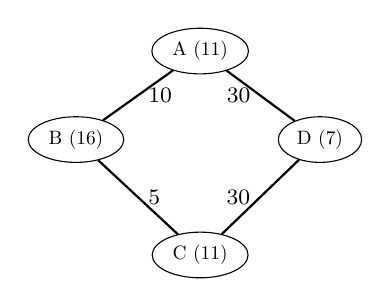
\begin{tikzpicture}
\usetikzlibrary{arrows}
\usetikzlibrary{shapes}
\tikzstyle{every node}=[draw, ellipse, minimum size=10pt,align=center,scale=0.7]
\node at (0,0)(1){A (11)};
\node[below left=1cm of 1](2){B (16)};
\node[below right=1cm of 1](4){D (7)};
\node[below=2cm of 1](3){C (11)};
\path[every node/.style={font=\footnotesize},thick]
    (1) edge node[right] {10} (2)
	edge node[left] {30} (4)
    (2) edge node[right] {5} (3)
    (4) edge node[left] {30} (3);
\end{tikzpicture}
  \end{subfigure}  
  \begin{subfigure}[b]{0.53\linewidth}
  \centering
  \subcaption{Virtual Network}\label{fig:Virtual}
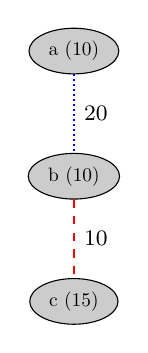
\begin{tikzpicture}
\usetikzlibrary{arrows}
\usetikzlibrary{shapes}
\tikzstyle{every node}=[draw, ellipse, fill=gray!40, minimum size=10pt, align=center, scale=0.7]
\node at (0,0)(1){a (10)};
\node[below=1cm of 1](2){b (10)};
\node[below=1cm of 2](3){c (15)};
\path[every node/.style={font=\footnotesize},thick]
    (1) edge[blue,densely dotted] node[right,color=black] {20} (2)
    (2) edge[red,thick,dashed] node[right,color=black] {10} (3);
\end{tikzpicture}
  \end{subfigure}   
\caption*{Source: from author (2015).}\end{figure}


\begin{figure}[!h]
  \centering
  \caption{Optimal solution for instance of Figure~\ref{fig:input}.\label{fig:mapping}}   
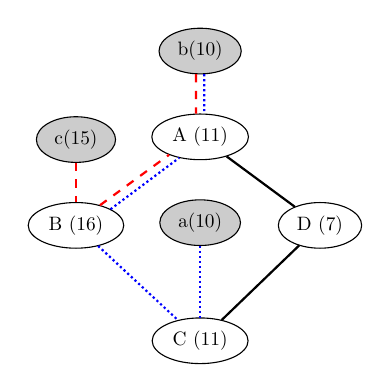
\begin{tikzpicture}
\usetikzlibrary{arrows}
\usetikzlibrary{shapes}
\tikzstyle{every node}=[draw, ellipse, minimum size=10pt,align=center,scale=0.7]
\node[fill=gray!40] at (0,0)(6){b(10)};
\node[below=0.5cm of 6] (1){A (11)};
\node[below left=1cm of 1](2){B (16)};
\node[below right=1cm of 1](4){D (7)};
\node[below=2cm of 1](3){C (11)};
\node[fill=gray!40, below=0.5cm of 1] (5){a(10)};
\node[fill=gray!40, above=0.5cm of 2] (7){c(15)};
\path[every node/.style={font=\footnotesize},thick]
    (5) edge[blue,densely dotted] node [] {} (3)
    (7) edge[red,dashed] node [] {} (2)
    (1) edge node [] {} (4)
    (2) edge[blue,densely dotted] node [] {} (3)
    (4) edge node [] {} (3);
  \draw[blue,thick,densely dotted] (2.25) -- (1.-135);
  \draw[red,thick,dashed] (2.40) -- (1.-150);
  \draw[blue,thick,densely dotted] (6.-80) -- (1.80);
  \draw[red,thick,dashed] (6.-100) -- (1.100);
\end{tikzpicture}
\caption*{Source: from author (2015).}\end{figure}

\section{Models}
\label{sec:models}
Most exact algorithms in the literature for the VNEP are based on ILP models. The following ILP model is based on~\cite{Alkmim2013}. It is adapted to the set of constraints presented in this work: let the decision variables $x_{v,s} = 1$ iff the substrate node $s$ hosts the virtual node $v$. And let $y_{v,w,s,j} = 1$ iff the physical link $(s,j)$ hosts the virtual link $(v,w)$.

\begin{align}
    \min & \sum\limits_{(s,j) \in E^{S}} \sum\limits_{(v,w) \in E^{V}} B_{v,w} y_{v,w,s,j} \label{eq:z} \\
    s.t. & \sum\limits_{v \in V^{V}} C_{v} x_{v,s} \leq C_{s}                     & \forall s \in V^{S}  \label{eq:flowcap} \\
    & \sum\limits_{s \in V^{S}} x_{v,s} = 1                                  & \forall v \in V^{V}  \label{eq:flowvirone}\\
         & \sum\limits_{v \in V^{V}} x_{v,s} \leq 1                               & \forall s \in V^{S} \label{eq:flowsubone}\\
         & \sum\limits_{j \in V^{S}} y_{v,w,s,j} - \sum\limits_{j \in V^{S}} y_{v,w,j,s} =  x_{v,s} - x_{w,s}  & \forall (v,w) \in E^{V}, s \in V^{S}\label{eq:flowflow} \\
         & \sum\limits_{(v,w) \in E^{V}} B_{v,w} y_{v,w,s,j} \leq B_{s,j}  & \forall (s,j) \in E^{S} \label{eq:flowbandwidth} \\
         & x_{v,s} \in \{0,1\} & \forall v \in V^{V}, s \in V^{S} \\
         & y_{k,l,m,n} \in \{0,1\} & \forall (k,l) \in E^{V}, (m,n) \in E^{S}
\end{align}

The objective function~\eqref{eq:z} minimizes the amount of bandwidth used by the virtual network. Constraints~\eqref{eq:flowcap} ensure that the capacities of substrate nodes are not surpassed. Constraints~\eqref{eq:flowvirone} and~\eqref{eq:flowsubone} enforce, respectively, that every virtual node is mapped to a different substrate node and every substrate node hosts at most one virtual node. Constraints~\eqref{eq:flowflow} are path constraints, they ensure that every virtual link is mapped to a path in the substrate graph. Finally, Equations~\eqref{eq:flowbandwidth} guarantee that the bandwidth capacities of physical edges are not violated.

Let us call this model \textbf{Compact Model} in contrast with the large model that will be presented later in this section.
As the VNEP is NP-Complete (a proof is given in Section~\ref{sec:complexity}), solving this ILP model is NP-Complete.
Branch \& Bound algorithms use linear relaxations to obtain bounds on optimal integer solutions.
The first problem with using the linear relaxation of the Compact Model is that there is no efficient algorithm to obtain integer solutions from that relaxation (proof in Section~\ref{sec:complexity}).
The second problem is that this relaxation provides a poor lower bound for the optimal solution, what has a negative impact on the performance of a Branch \& Bound algorithm.
It is always possible to obtain a solution with cost zero for the relaxation of this model.

\begin{proposition}
There is always a solution with cost zero to the compact model.
\end{proposition}

\begin{proof}
If every $x_{vs}$ is set to~$1 / |V^S| $, all constraints are respected and the left hand side of Constraints~\eqref{eq:flowflow} is zero. 
Therefore all variables $y_{vwsj}$ can be set to zero.
Hence, the cost of the optimal solution for the relaxed problem is always zero, resulting in a trivial lower bound.
\end{proof}
\vspace{-0.5cm}

\begin{comment}
Models based on Dantzig-Wolfe decomposition usually provide better lower bounds than compact models.
Also, the structure of the problem can be better exploited, resulting in a more efficient exploration of the solution space.

The Compact Model has a $p$-block angular structure, i.e., the model can be decomposed into $p$ independent blocks and $p$ linking blocks.
A $p$-block angular structure is illustrated in Figure~\ref{eq:pblock}.
Constraints~\eqref{eq:flowflow} present this kind of structure: each virtual link is independent of the other virtual links in those constraints and they are linked by Constraints~\eqref{eq:flowbandwidth}.
Thus, the problem can be decomposed in $|E^V|$ independent problems.
Each problem corresponds to a single virtual link mapping problem.

\begin{equation}
A = \left[  \begin{array}{cccc}
            A_{1} & A_{2} & \ldots & A_{p} \\
            B_{1} &       &        &       \\
                  & B_{2} &        &       \\
                  &       & \ddots &       \\
                  &       &        & B_{p} \\
            \end{array} \right] \label{eq:pblock}
\end{equation}

The polyhedron defined by the compact model is bounded, since all variables are binary, and it is nonempty (a two-phase method is used to guarantee that there is always a solution, c.f. Chapter~\ref{ch:cg}).
A nonempty and bounded convex polyhedron can be represented by a convex combination of its extreme points \cite{lasdon1970}.
Thus, let $C$ be the polyhedron defined by the Compact Model, any element $y \in C$ can be represented as:

\begin{align}
  y = & \sum\limits_{ j } \lambda_{j} x^{j} & \\
  where   & \sum\limits_{j} \lambda_{j} = 1 & \\
          & \lambda_{j} \geq 0              &
\end{align}

Where the $x^{j}$ are all the extreme points of polyhedron $C$.

Therefore, using Dantzig-Wolfe decomposition, we can reformulate the Compact Model as follows: Choose, from all valid paths, those that minimize the objective function. We follow to define a model based in paths that cover virtual links.

\begin{definition}
A substrate path $p = w_{1}, w_{2},\ldots, w_{n}$ ($w_{i} \in V^S, \forall i \in [n]$) \textbf{covers} the virtual link~$(u,v)$ if every edge in the path has enough capacity to host the virtual link, the first node $w_{1}$ in the path has enough CPU capacity to host virtual node $u$, and the last node $w_{n}$ has enough capacity to host the virtual node $w$.
\end{definition}

Let $P^k$ be the set of all paths in the physical network that cover the virtual link $k$.
We can write every $y_{k}$ as a convex combination of extreme points~$\{\delta_p\}_{p \in P^k}$.

\begin{align}
  y_{k} = & \sum\limits_{p \in P^{k}} \delta_{p} z_{p} \label{eq:yk} & \\
        %& x_{v,s} = \sum\limits_{(v,w) \in E^V} \sum\limits_{p \in P^{(v,w)}} \delta_{v,s,p} z_{p}
          & \sum\limits_{p \in P^k} z_{p} = 1 & \forall k \in E^V \\
          & z_{p} \in \{0,1\}                       & \forall k \in E^V, p \in P^k
\end{align}

%\begin{align}
%  s.t.  & \sum\limits_{p \in P^{k}} z_{p} = 1, z_{p} \geq 0 
%\end{align}

Therefore, each variable $y_{v,w,s,j}$ is uniquely defined in terms of paths in the graph as follows:

\begin{equation}
  y_{v,w,s,j} = \sum\limits_{p \in P^{(v,w)}} \delta_{s,j,p} z_{p} \label{eq:definition}
\end{equation}

Where $\delta_{s,j,p}$ is set to one iff the path $p$ contains the physical edge $(s,j)$.

If we replace the variables $y_{v,w,s,j}$ with variables $z_{p}$ in Constraints~\ref{eq:flowflow}:

\begin{align}
  \sum\limits_{j \in V^{S}} \sum\limits_{p \in P^k} \delta_{s,j,p} z_{p} - \sum\limits_{j \in V^{S}}\sum\limits_{p \in P^k} \delta_{j,s,p} z_{p} = x_{v,s} - x_{w,s}     & \quad \forall (v,w) = k \in E^{V}, s \in V^{S} \label{eq:flowwithpathvar}
\end{align}

Let $p = v_{1},v_{2},\ldots,v_{n}$ be a path in the substrate graph. Since $p$
is an undirected path in a graph, with exception of $j = v_{1}$ and $ j = v_{n}$,
the right hand side of the above equation is equal 
to zero. So this equation is equivalent to:

\begin{align}
  \sum\limits_{p \in P^k : (v,s) \in p} z_{p}
    - \sum\limits_{p \in P^k : (s,w) \in p} z_{p} 
    = x_{v,s} - x_{w,s}   
    & \quad \forall (v,w) = k \in E^{V}, s \in V^{S} \nonumber % \label{eq:flowwithpathvar}
\end{align}

These constraints guarantee that if a virtual node $v$ is mapped to a node $s$, only paths that map $v$ to $s$ are used. They can be replaced by the following equation:

% begin comment
If for every $v \in V^S$ we sum the equation above we obtain:

\begin{align}
  \sum\limits_{(v,w) = k \in \delta(v)}\sum\limits_{p \in P^k : (v,s) \in p} z_{p}
    - \sum\limits_{(v,w) = k \in \delta(v)}\sum\limits_{p \in P^k : (s,w) \in p} z_{p} & \nonumber \\
    = |\delta(v)| x_{v,s} - \sum\limits_{(v,w) \in E^{V}} x_{w,s}       & \quad \forall v \in V^{V}, s \in V^{S} \label{eq:aggreg}
\end{align}

Since every path is valid, no path would map both $v$ and $w$ to $s$, so $\sum\limits_{(v,w) = k \in E^V}\sum\limits_{p \in P^k : (s,w) \in p} z_{p}$ is equal to zero.

Since by Equation~\ref{eq:flowsubone} and by the integrality property of the decision variables, the right
hand-side of the equation can be either zero or one. The equation holds in both of those cases.
If it is zero, the right hand side of \eqref{eq:flowwithpathvar} is non-negative, so
the left hand-side of that equation is also non-negative. If it is one, the left hand-side
can be at most one, so the equation also holds, therefore in all cases the equation is positive.
Therefore the left-hand side of \eqref{eq:aggreg} is always smaller than the right hand side and the 
Equation~\eqref{eq:final} holds for any $M \geq \delta(v)$.

\begin{align}
    \sum\limits_{(v,w) \in E^{V}} x_{w,s} = 
    \sum\limits_{(v,w) = k \in E^{V}}\sum\limits_{p \in P^k : (s,w) \in p} z_{p} & \quad \forall v \in V^{V}, s \in V^{S}
\end{align}
%end comment

\begin{align}
  \sum\limits_{k \in E^{V}}\sum\limits_{p \in P^k : (v,s) \in p} z_{p} \leq M x_{v,s}       & \quad \forall v \in V^{V}, s \in V^{S}
  \label{eq:final}
\end{align}

Where $M$ is a number larger than or equal to the maximum degree of the virtual network. Thus, if $x_{v,s}$ is set to zero, no path that maps $v$ to $s$ can be used.

Therefore, replacing variables $y$ by the new decomposed variables $z$ in the compact model, we obtain the flow-based Model (note that Constraints \eqref{eq:flowcap} could be omitted, since they are by definition respected):
\end{comment}

In order to improve the lower bound given by the linear relaxation of the compact model, VNEP can be modeled in terms of paths in the auxiliary graph. 
Two sets of decision variables are used. For each $v \in V^{V}$ and $s \in V^{S}$, the variable $x_{vs} \in \{0,1\}$ is set to one iff the substrate node $s$ hosts the virtual node~$v$. 
Likewise, for each path $p$ in the set of all paths $P$, the variable $z_{p} \in \{0,1\}$ is set to one if the path is used in the VNEP. 
For each path~$p$, the input data $\delta_{e,p}$ is one if the physical edge~$e$ is in the path~$p$, and zero otherwise.
For each virtual link $k=(v,w) \in V^V$, $P^k$ is the set of all simple paths in the substrate graph whose endpoints have enough CPU capacity to host $v$ and $w$, and whose links have enough capacity to host $k$.
The set of Constraints~\eqref{eq:flowcap} of the compact model can be omitted because only paths that attend this constraint are part of the model.
The objective function is the minimization of the total bandwidth used by the virtual network. 
If a path $p$ serves a virtual link $k$, the cost of this path $c_{p}$ is defined as the number of physical edges in the path.
The \textbf{Flow-based Model} for the single-path VNEP is presented below:


\begin{align}
  \min  & \sum\limits_{k \in E^{V}}\sum\limits_{p \in P^k}  c_{p} B_k z_{p} \label{eq:obj} \\
        & \sum\limits_{s \in V^{S}} x_{v,s} = 1                                  & \forall v \in V^{V} \label{eq:virone} \\
        & \sum\limits_{v \in V^{V}} x_{v,s} \leq 1                               & \forall s \in V^{S} \label{eq:subone} \\
        & \sum\limits_{k \in E^{V}}\sum\limits_{p \in P^{k}} \delta_{e,p} B_{k} z_{p} \leq B_{e} & \forall e \in E^{S} \label{eq:bandwidth} \\
        & \sum\limits_{k \in E^{V}}\sum\limits_{p \in P^k : (v,s) \in p} z_{p} \leq M x_{v,s} & \forall v \in V^{V}, s \in V^{S} \label{eq:onlyoneaux}\\
        & \sum\limits_{p \in P^{k}} z_{p} = 1                                    & \forall k \in E^{V} \label{eq:virdemone} \\
        &  x_{v,s} \in \{0,1\}  & \forall v \in V^{V}, s \in V^{S} \nonumber \\
        & z_{p} \in \{0,1\}    & \forall p \in {P} \nonumber
\end{align}

Constraints~\eqref{eq:virone} ensure that all virtual nodes are mapped. Each substrate node can host at most one virtual node~\eqref{eq:subone}.
Constraints~\eqref{eq:virdemone} state that all virtual links have to be mapped to a single path in the substrate graph.
Constraints~\eqref{eq:bandwidth} ensure that the bandwidth constraints are not violated.
Finally, let M be the greatest degree of the virtual network, Constraints~\eqref{eq:onlyoneaux} enforce that only one auxiliary edge is used for each virtual node.

Solving the problem using decomposition introduces a large number of new variables. However, the relaxation of the flow-based Model provides better lower bounds and, since it uses the structure of the problem directly, we can obtain more information about the problem with relaxed solutions.

\begin{comment}
\section{Bounds on Optimal Solutions}
\label{sec:bounds}
The use of lower bounds can drastically reduce the running time of exact exponential algorithms. The closer the bound to the optimal solution, the more branches are pruned on the search tree.

Let the optimal solution of a given instance $I$ of the VNEP be $OPT(I)$. Since every virtual link has to be mapped to a path in the substrate network, a lower bound on the optimal solution is the sum of all the edge demands in the virtual network. As the graph has a limited capacity on the substrate network edges, a natural upper bound is the sum of all capacities. Those two bounds are formalized in the Equation~\ref{eq:lb1}.

\begin{equation}
  \sum\limits_{e \in E^{V}} B_{e} \leq OPT(I) \leq \sum\limits_{e \in E^{S}} B_{e}
  \label{eq:lb1}
\end{equation}

A better lower bound is given by Equation~\ref{eq:lb2}. Let $dist(s, t)$ be the minimum size in numbers of edges of all simple paths in the substrate network from $s$ to $t$.

\begin{equation}
  \sum\limits_{\forall(v,w) = k \in E^{V}} 
  ( \min\limits_{\forall s,t \in V^{S} | C_{v} \leq C_{s}, C_{w} \leq C_{t} } \{ dist(s,t) \} 
  B_{k} ) \leq OPT(I) \label{eq:lb2}
\end{equation}

The lower bound in Equation~\ref{eq:lb2} can be obtained in time $O(|E^{S}||V^{S}|)$ by running one breadth-first search for each node.

This lower bound can be improved by replacing $dist(s, t)$ by $cap\_dist(s, t, B_{k})$. Where the latter provides the number of edges of shortest path between $s$ and $t$ where every physical edge has a capacity of at least $B_{k}$. This improvement incurs in an increase in the complexity of obtaining it.
\end{comment}

\section{Complexity}
\label{sec:complexity}

%Several heuristics were developed for the VNEP, but none of them is guaranteed to find a feasible solution. 
We show in this section that %there could not exist an efficient algorithm that always finds a feasible solution 
%(not necessarily the optimal solution) unless $P=NP$, and then there is no approximation algorithm for the VNEP.
%Initially we show that 
the VNEP problem is NP-Hard by a reduction from the Bin Packing Problem (BPP), which is a classical NP-Complete problem.
The VNEP was previously shown to be NP-Hard by a reduction from the Unsplittable Flow Problem~\cite{Yu2008}, 
but by the reduction from the BPP we further show it does not exist an algorithm that is guaranteed to generate a feasible solution unless P=NP, and then VNEP cannot be approximated.

The Bin Packing Problem has as input a set~$N$ of items and a bin size of capacity~$B$.  Each item~$i$ has a weight~$w_{i} \leq B$. The goal is to fit all items using the minimum number of bins, respecting their capacities. The decision version asks if it is possible to fit all items in at most $k$ bins.


Any instance $I$ of the BPP can be transformed into an instance of the VNEP through the procedure $\phi$, which generates a virtual and physical graphs as described next.
%First we show that $\phi$ is polynomial in the size of $N$, then we show that a polynomial algorithm that finds a feasible solution for the VNEP provides a polynomial algorithm for the B\&P. 
%By the transformation, a physical substrate graph is created with $2|N| + 2k$ nodes and $2|N|k + k$ edges, and a virtual network graph is created with $2|N|$ nodes and $2n - 1$ edges, as described next. 
%This new instance is created in such a way that there is a feasible solution for the VNEP instance $\phi(I)$ iff there is also a solution for instance $I$. Therefore an algorithm that finds any feasible solution for the VNEP solves B\&P.

\textbf{Virtual Network:} For each item $i \in N$, two nodes are created: one with demand three and another with demand two. 
Those nodes are linked with virtual links with bandwidth $w_{i}$. 
Moreover, nodes corresponding to items $i$ and $i+1$ for every $i < |N|$ are linked to assure the connectivity of the network.
Their demand is not important and are set to zero.

\textbf{Physical Substrate Network:} For each item $i \in N$ two nodes are created, one with capacity three and another with capacity two. 
Furthermore, $2k$ nodes are created with capacity one. 
For convenience, let us call nodes with capacity three the upper nodes, nodes with capacity two the lower nodes, and nodes with capacity one the middle nodes, in the physical and virtual networks.
Each upper node is linked with $k$ middle nodes, the rest of the $k$ middle nodes is linked with all lower nodes. 
Each of the~$k$ middle nodes linked with the upper nodes are linked with one single middle node which is linked to the lower nodes. 
Capacities of all edges are set to~$B$, the bin size.

An example of this transformation is show in Figures~\ref{fig:transvir} and~\ref{fig:transsub}. 
The original BPP consists of three items of weights three, four, and eight, and $B=8$. 
The value of $k$ in the decision version is set to two. 
A solution is given by mapping the virtual links with weights three and four on physical edges on the left-central, 
and the other virtual link of weight eight into the edge on the right-central.

\begin{figure}[!h]
  \centering
  \caption{Virtual Graph resulted from transformation $\phi$.}\label{fig:transvir}
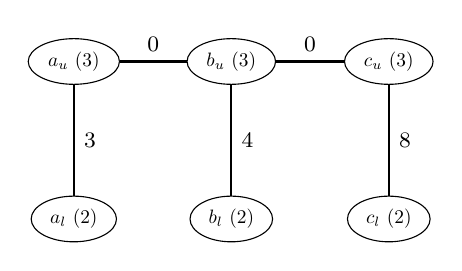
\begin{tikzpicture}
\usetikzlibrary{arrows}
\usetikzlibrary{shapes}
\usetikzlibrary{graphs}
\tikzstyle{every node}=[draw, ellipse, minimum size=10pt,align=center,scale=0.7]
\node at (0,2)(1){$a_{u}$ (3)};
\node at (2,2)(2){$b_{u}$ (3)};
\node at (4,2)(3){$c_{u}$ (3)};
\node at (0,0)(8){$a_{l}$ (2)};
\node at (2,0)(9){$b_{l}$ (2)};
\node at (4,0)(10){$c_{l}$ (2)};
%  \draw (1) -- (4) node [below]{8};

\path[every node/.style={font=\footnotesize},thick]
    (1) edge node[right] {3} (8)
    (2) edge node[right] {4} (9)
    (3) edge node[right] {8} (10)
    (1) edge node[above] {0} (2)
    (2) edge node[above] {0} (3);
\end{tikzpicture}
\caption*{Source: from author (2015).}\end{figure}

\begin{figure}[!h]
  \centering
  \caption{Substrate Graph resulted from transformation $\phi$.}\label{fig:transsub}
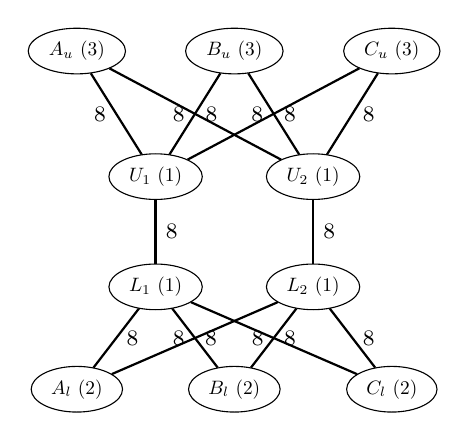
\begin{tikzpicture}
\usetikzlibrary{arrows}
\usetikzlibrary{shapes}
\usetikzlibrary{graphs}
\tikzstyle{every node}=[draw, ellipse, minimum size=10pt,align=center,scale=0.7]
\node at (0,3)(1){$A_{u}$ (3)};
\node at (2,3)(2){$B_{u}$ (3)};
\node at (4,3)(3){$C_{u}$ (3)};
\node [below=0.3cm of 3] at (1,2)(4){$U_{1}$ (1)};
\node [below=0.3cm of 3] at (3,2)(5){$U_{2}$ (1)};
\node [below=0.7cm of 4] at (1,1)(6){$L_{1}$ (1)};
\node [below=0.7cm of 4] at (3,1)(7){$L_{2}$ (1)};
\node [below=1cm of 7] at (0,0)(8){$A_{l}$ (2)};
\node [below=1cm of 7] at (2,0)(9){$B_{l}$ (2)};
\node [below=1cm of 7] at (4,0)(10){$C_{l}$ (2)};
%  \draw (1) -- (4) node [below]{8};

\path[every node/.style={font=\footnotesize},thick]
    (1) edge node[left] {8} (4) 
    (1) edge node[right] {8} (5)
    (2) edge node[left] {8} (4)
    (2) edge node[right] {8} (5)
    (3) edge node[left] {8} (4)
    (3) edge node[right] {8} (5)
    (4) edge node[right] {8} (6)
    (5) edge node[right] {8} (7)
    (8) edge node[right] {8} (6)
    (8) edge node[right] {8} (7)
    (9) edge node[left] {8} (6)
    (9) edge node[right] {8} (7)
    (10) edge node[left] {8} (6)
    (10) edge node[right] {8} (7);
\end{tikzpicture}
\caption*{Source: from author (2015).}\end{figure}

\begin{lemma} \label{lem:reduction}
  Any Bin Packing instance can be reduced to an instance of the Virtual Network Embedding Problem through procedure $\phi$.
\end{lemma}

\begin{proof}
There are~$n$ virtual nodes with demand three and~$n$ physical nodes with capacity three, therefore any feasible solution would map all virtual upper nodes to physical upper nodes. Likewise for physical and virtual nodes with capacity and demand two.
Hence, in the instance~$\phi(I)$ there is always a feasible mapping of the nodes.
Moreover, each of the~$n$ edges has to be mapped to a single path in the substrate graph between the upper nodes and the lower nodes.
Additionally, every path has to contain at least one edge between the middle nodes.
Those edges represent bins.
Mapping virtual links to those edges is tantamount to fit items in a bin.
%Hence, if a solution for $\phi(I)$ is given, a solution for $I$ can be obtained by selecting the first of the middle edges (the edges that link the middle nodes) in the $n$ paths.
%Moreover, if there is any feasible mapping for $\phi(I)$, the answer for the B\&P decision version is YES. 
%Therefore, if a polynomial algorithm exists that solves $\phi(I)$, we can use it to compute the answer to $I$ in polynomial time.
\end{proof}


\begin{lemma} \label{lem:transpol}
  The transformation $\phi(I)$ is polynomial in $|N|$.
\end{lemma}

\begin{proof}
The transformation $\phi$ creates two graphs, one with $2|N| + 2k$ nodes and $2|N|k + k$ edges and another with $2|N|$ nodes and $2n - 1$ edges. 
As $k < |N|$, and every item fits into a single bin, the size of the VNEP instance is limited polynomially by $|N|$, the number of items of $I$.
\end{proof}

\begin{lemma} \label{lem:polapp}
  If there exists a polynomial time algorithm that finds a feasible solution for $\phi(I)$, there is a polynomial time algorithm that finds a feasible solution for $I$.
\end{lemma}

\begin{proof}
All virtual nodes with demand three have to be mapped to substrate nodes with capacity three.
If one of the nodes of demand two is mapped to a substrate node of capacity three, there will be an unmapped virtual node of capacity three. 
Likewise, for nodes of capacity two.
%as there are only $|N|$ substrate nodes with capacity two, every one of the $|N|$ virtual nodes with demand two will be mapped to a substrate node of capacity two. 
Therefore there is always a feasible node mapping for $\phi(I)$. 
Note that the mapping order is not important: any virtual node with demand $x$ can be mapped to any physical node with capacity $x$.

If there is a feasible mapping for the virtual network of $\phi(I)$, the answer to I is YES:
Given a feasible mapping $M$, all virtual edges are mapped to a path in the substrate graph. 
Let $p_{i}$ be the path for which the virtual link~$i$, corresponding to the item~$i$, was mapped to. 
Let $j$ be the first substrate edge in $p_{i}$ that links the middle nodes. The edge~$j$ corresponds to the bin~$j$. Thus a solution for $I$ can be constructed if item~$i$ is allocated into bin~$j$. 
Since the capacity of all edges are not surpassed, the $k$~bins can hold the $|N|$~items.

If the answer for I is YES, there is a feasible mapping for $\phi(I)$:
Suppose that there is a configuration of the items into $k$ bins.
A solution for $\phi(I)$ can be constructed from a solution for $I$.
Suppose any feasible mapping $M$ of nodes for the virtual network (as it was shown before, there always exists a feasible mapping of nodes).
Let $f_{M}(u)$ be the substrate node for which the virtual node $u$ is mapped. 
Every virtual link $(u,v)$ corresponding to the item $i$ is mapped to the path $(f_{M}(u), x)$, $(x,y)$, $(y,f_{M}(v))$, where $(x,y)$ is the substrate edge corresponding to the bin $j$ for which the item $j$ was allocated in the solution for $I$.
Since the sum of the items in a bin $j$ does not exceed the capacity $B$, every virtual link can be mapped in the physical graph.
\end{proof}

\begin{lemma} \label{lem:cert}
  VNEP is an NP problem
\end{lemma}

\begin{proof}
  A solution for a VNEP instance I can be verified in polynomial time in the size of the instance. For every virtual node $u$ it suffices to check if the physical node $f_v(u)$ has enough capacity to host it, for every virtual link $(u,w)$ it suffices to check the path $p = f_e(u,w)$ is indeed a path (every adjacent edge shares one endpoint), and for every physical edge $e$, if all the links that are mapped in $e$ do not surpass its capacity.
\end{proof}

\begin{theorem} \label{th:npcomplete}
  VNEP is an NP-Complete problem.
\end{theorem}

\begin{proof}
The hardness of the VNEP problem follows from Lemmas~\ref{lem:reduction}-\ref{lem:cert}. 
\end{proof}

\begin{corollary} \label{co:nopoly}
  There is no polynomial time algorithm that finds a feasible solution for VNEP, unless $P=NP$.
\end{corollary}

\begin{proof}
  Suppose there is a polynomial time algorithm that finds a feasible solution (not necessarily optimal) for VNEP. From~\ref{lem:polapp}, it follow that there is a polynomial algorithm for solving BPP\@. 
  But this is only possible if $P = NP$.
\end{proof}

Corollary~\ref{co:nopoly} implies that there is probably no time efficient approximation algorithm for VNEP, since such an algorithm would provide a polynomial time algorithm to solve BPP.


\section{Column Generation for the VNEP with unsplittable paths}

\begin{figure}[h]
  \centering
  \includegraphics[scale=0.55]{cgpathcex.pdf}
  \caption{Auxiliary graph, invalid path example.}\label{fig:auxcex}
\end{figure}

\subsection{Preliminary Tests}
Four sets of instances were generated. The number of nodes of the physical substrate networks range from 10 to 50, and of the virtual networks range from 2 to 15.

\begin{center}
\begin{tabular}{l l l}
Set id    & capacity    & demand      \\
\hline
set 1     & $[20,40]$ & $[10,25]$   \\
set 2     & $[15,40]$ & $[15,25]$   \\
set 3     & $[15,40]$ & $[15,35]$   \\
set 4     & $[10,40]$ & $[10,40]$   \\
\end{tabular}
\end{center}


\chapter{Branch \& Price}
\label{ch:bp}

The column generation (CG) algorithm solves only the linear relaxation of the problem.
To obtain integer solutions for the VNEP, CG is embedded in a Branch \& Bound algorithm (B\&B).
A B\&B algorithm where each node is solved through a column generation is called Branch \& Price (B\&P).

We implemented a classic B\&P procedure which is summarized in Algorithm~\ref{alg:bp}.
Initially, the relaxation of the problem is solved.
If the optimal solution is not integral, the problem is split into two subproblems.
This process is called branching (Section~\ref{sec:branching}).
These subproblems are inserted in a priority queue with the key set to their relaxation value.
At each iteration, a subproblem is selected (Section~\ref{sec:nodesel}) from the queue and solved through a CG algorithm.
To speed up the algorithm by improving upper bounds, a constructive solution is build at each iteration (Section~\ref{sec:heur}) aiming to obtain an integral solution.
In case the incumbent integral solution has a better objective value than a subproblem relaxation, that branch is not expanded anymore since the relaxation of the problem is a lower bound on the integral solution.

\begin{algorithm}[t]
\caption{Branch \& Price Algorithm}
$Q$ = {relaxation of IP}

\While{$Q$ is not empty}
  {
    subproblem = select\_node($Q$)\; \label{alg:genbp:snode}
    $x^*$ = solve subproblem using column generation\;
    \If{feasible($x^*$) and $\phi(x^*) < UB$}
    {\eIf{$x^*$ is integral}
      {$UB = \phi(x^*)$\;}
      {build heuristic solution\;
      split subproblem into subproblems and add them to $Q$\;\label{alg:bp:split}}
    }
  }
\label{alg:bp}
\end{algorithm}

The problems are branched with the introduction of cuts. Those cuts can turn the problem infeasible. 
New columns have to be inserted in order to make the problem feasible again.
The two-phase approach explained in Chapter~\ref{ch:cg} is used to overcome this problem.

Next we describe decisions taken by the B\&B for the VNEP we have implemented.

\section{Branching}
\label{sec:branching}
%A solution is fractional if one or more variables have a fractional value.
When expanding a node of the B\&B tree, if the solution is fractional, a variable is selected to be branched (Section~\ref{sec:varsel}).
The model solved at each node has two sets of decision variables: node mapping variables $x_{v,s}$ and path mapping variables $z_{p}$.
The former has a fixed size, while the latter grows during B\&P execution.
Therefore each one is treated differently. 

\subsection{Variable Selection}
\label{sec:varsel}
Variables $x_{v,s}$ are intregralized first starting with variable with values closest to $0.5$.
Once all variables $x$ are integral, path variables $z_{p}$ are verified in order of the origin node label.
Paths with the same origin are verified in the order they were generated. 

\subsection{Node mapping branching}
We tested two methods of branching for variables $x_{v,s}$.
In the first, two subproblems are created, one for which the substrate node $s$ is forbidden of hosting $v$ ($x_{v,s} \leq 0$) and another for which the node $s$ is forced to host $v$ ($v_{v,s} \geq 1$).
The second is called Generalized Upper Bound (GUB):
since $\sum\limits_{s' \in V^S} x_{v,s'} = 1$, one can cut more than one variable at a time. Two problems are created, one of which half the variables $x_{v}$ are forbidden by adding the cut $\sum\limits_{s < |V^S| / 2} x_{v,s} \leq 0$, and another for which the other half of variables are forbidden.
In both methods, the addition of cuts affect the pricing problem.
The auxiliary edge $(v,s)$ is either forbidden or fixed accordingly.

\subsection{Path branching}
Branching of path variables is not as straightforward as branching node variables. 
Individually branching on path variables would yield a large number of nodes to explore, since the number of paths grows exponentially with the size of the instance. 
To avoid this problem, paths are branched by introducing constraints that simulate restrictions on variables $y$ from the compact model. 
Suppose that for a given node, there exists one path variable $z_{p}$ that has a fractional value. Then there must be at least another variable $z_{p'}$ that is also fractional, since the sum of the variables that cover a virtual link is $1$. 
The paths $p$ and $p'$ associated to variables $z_{p}$ and $z_{p'}$ must have at least two different substrate edges $e \in p, e \notin p'$ and $f \in p', f \notin p$, otherwise they would be the same path. Then, two branches are generated, one with $e$ forbidden to belong to the path, and another for which $f$ is forbidden. Edges are not fixed, because it is easier to find a path that does not use multiple edges (it suffices to set their weights to a large value) than it is to fix edges. An edge $e$ is forbidden to be used to cover the virtual link $k$ by adding the cut $c(k,e) = \sum\limits_{p \in P^k} \delta_{e,p} z_p \leq 0$.

Adding these cuts affects the pricing problem. For each $k \in E^V$ and $e \in E^S$ a dual variable $\psi_{k,e}$ associated with the cut $c(k,e)$ is created. The values of these variables are added to the cost of each edge in the auxiliary graph. So each physical edge in the auxiliary graph has the cost $B_{k}(1 - y_{e} - \psi_{k,e})$.

\section{Node Selection}
\label{sec:nodesel}
The order in which active nodes are visited affects the performance of the algorithm. A balance has to be found between finding good upper bounds and visiting promising nodes. We tested three approaches: Depth First Search (DFS), Best First Search (BFS), and Best Projection (BPJ). DFS visits nodes in the order they are created. BFS visits first the most promising nodes, i.e., nodes with the lowest dual bound. BPJ visits nodes with fewer fractional variables first, since they are possibly closer to an integral solution.

\section{Heuristic Solution}
\label{sec:heur}
It was seen in Section~\ref{sec:complexity}, that to obtain a feasible solution for the VNEP is NP-Hard.
Nevertheless, a greedy algorithm can be applied and in many situations is able to find a feasible solution.
Moreover, if part of the solution is already fixed, only the remaining part has to be constructed.
This happens when a greedy solution is applied on a subproblem, which uses all variables set on that branch of the B\&B tree since the root node.
Constructed feasible solutions can improve upper bounds allowing to prune entire branches of the B\&P search tree.

A solution obtained by the column generation may contain several fractional variables. 
The values of those variables contain valuable information about the problem. 
Each virtual node $v$ is mapped to the free physical node $s$ for which the value of $x_{v,s}$ is the largest. 
After all nodes are mapped, a breadth first search is used to map virtual links to paths in the physical substrate graph. The mapping of edges can fail if no path with enough bandwidth is found.

This algorithm is applied at each node of the B\&B tree. If a feasible solution is successfully built by the constructive heuristic algorithm, and the obtained solution is better than the current upper bound, the incumbent solution is updated.



\chapter{Experimental Results}
\label{ch:results}


This section presents an experimental evaluation of the proposed B\&P algorithm. 
Results from B\&B are compared with results from the compact model presented in Section~\ref{sec:models} solved with CPLEX\@. 
Four aspects of the algorithm are tested: the time spent to find the first integral solution, the running time, the number of instances solved, and the quality of solutions that were not proved to be optimal due to a time limit constraint. 
All tests were performed on a processor Intel Core i7 930 with 12 Gb of memory using a single thread. The commercial solver CPLEX 12.5 was used to solve the relaxed and integer models. All running times are in seconds, and a time limit of one hour was used in all runs.


\section{Datasets}
\label{sec:datasets}

As virtualization is a fairly recent field, there is no established set of benchmark instances available for the VNEP\@.
The properties of physical substrate networks and virtual network embedding requests are not well understood~\cite{Chowdhury:2012}. Hence most works use synthetic networks \cite{FischerSurvey}.
Following this approach, all instances used in this experimental evaluation are generated with the GTI-ITM tool~\cite{Zagura:1996}.
This tool is capable of generating graphs with three different topologies: random, hierarchical and transit-stub. Figure~\ref{fig:topo} presents an illustrative example of each topology.

Random instances are generated by spreading the nodes randomly in a 100 by 100 plane. These nodes are randomly linked using Waxman model \cite{Zagura:1996}. In this model, the probability of connecting two edges is $\alpha e^{- d / (100 \beta)}$, where $d$ is the Euclidean distance between the nodes, and $\alpha$ and $\beta$ are parameters. Thus, a larger $\alpha$ means a denser graph, and a larger $\beta$ means longer edges in the graph. Two types of random instances are generated: \textbf{Dense Random}, using $\alpha = 0.8$ and \textbf{Sparse Random}, using $\alpha = 0.5$. 
Both sets use $\beta = 0.2$.


\textbf{Hierarchical} instances are generated recursively. Initially, a random graph is created in a 100 by 100 plane. Then each node is replaced by a random graph with an average of five nodes. To generate those graphs the parameters $\alpha = 0.5$ and $\beta = 0.2$ were used.

\textbf{Transit-stub} is an hierarchical topology that best model the Internet~\cite{Zagura:1996}. Each node in a randomly generated graph is replaced by a subgraph called transit domain with an average of four nodes. To these domains are attached an average of three stub domains. Each stub domain has an average of two nodes. The transit domains as well as the stub domains are connected randomly with a probability $\alpha = 0.5$.

\begin{figure}
        \centering
        \caption{Topology examples}\label{fig:topo}
        \begin{subfigure}[b]{0.45\textwidth}
                \caption{Sparse Random}
                \includegraphics[width=\textwidth]{exsparse}
                \label{fig:gensparse}
        \end{subfigure}%
        ~ 
        \begin{subfigure}[b]{0.45\textwidth}
                \caption{Dense Random}
                \includegraphics[width=\textwidth]{exdense}
                \label{fig:gendense}
        \end{subfigure}

        \begin{subfigure}[b]{0.45\textwidth}
                \caption{Hierarchical}
                \includegraphics[width=\textwidth]{exhier}
                \label{fig:genhier}
        \end{subfigure}
        ~ 
        \begin{subfigure}[b]{0.45\textwidth}
                \caption{Transit-Stub}
                \includegraphics[width=\textwidth]{exts}
                \label{fig:gents}
        \end{subfigure}
\caption*{Source: from author (2015).}\end{figure}

Each instance is composed of one physical substrate graph of one of the four topologies (Dense Random, Sparse Random, Hierarchical, Transit-stub) and one Sparse Random virtual network.  Virtual networks were generated with connectivity 50\% as in \cite{Chowdhury:2012}. Capacities of physical nodes and edges are randomly generated integers in the interval $[1,100]$. Considering the demands of virtual networks, two sets of instances were generated: one with \emph{low demand} with demands in the interval $[1,25]$, and another with \emph{high demand} with demands in the interval $[25,100]$.

As one of the purposes of this study is to test the limits of exact algorithms, large physical networks were generated.
Instances were generated from 20 to 200 nodes for random sparse and random dense topologies (6 sizes of substrate networks each).
For hierarchical instances, from 125 to 250 nodes (6 sizes of substrate networks). 
For Transit-stub, graphs from 90 to 270 nodes (5 sizes of substrate networks).
Virtual networks are in general small, and were generated from 2 to 18 nodes considering all even sizes in this interval.
Input data for the problem was build considering all combinations of substrate and virtual networks, and for each combination two instances are build considering a low and high demands of the substrate network.
Thus, in overall 414 instances were tested.


In Section~\ref{sec:param} we describe the parameter setting, while that in Section~\ref{sec:bptest} we present the B\&P results, and compare against the ones found by the compact model solved with CPLEX. The amount of time spent by each component of column generation is analysed in Section~\ref{sec:pritime}

\section{Parameter Testing}
\label{sec:param}

As explained in the previous section, the node selection and branching methods influence the overall performance of the algorithm.
The use of the heuristic constructive method can also influence the performance of Branch \& Price.
The following experiments compare different options for these components considering one instance for each size in a total of 414 instances.
The main metric used is the running time to obtain the optimal solution and the number of instances solved optimally in the available time limit.
Initially we tested the performance of the B\&B algorithm selecting nodes using  $DFS$, $BFS$, and $BPJ$ and results are summarized in Table~\ref{tab:nodesel}. 
The table shows for each of the four sets of instances, the number of tested instances in column \textbf{\#inst}, and for each node selection method, the number of optimal solutions found within the time limit in column~\textbf{\#opt}, and the average running time in seconds in column~\textbf{time(s)}.

\begin{table*}[h]
\footnotesize
\begin{center}
  \caption{Node Selection Results}\label{tab:nodesel}
\begin{tabular} {l l | r r | r r | r r | r r }
\hline
                &                &  \multicolumn{2}{c|}{DFS}  & \multicolumn{2}{c|}{BFS}   & \multicolumn{2}{c|}{BPJ}  \\
  set           & \#inst           &  \#opt       & time(s)        & \#opt   & time(s)          & \#opt           & time(s)     & DFS $\sim$ BFS   & BPJ $\sim$ BFS  \\
 \hline 
 Random-Sparse  & 108            & 76         & 1086.20    & 85        & 851.90       & 83            & 863.66   & < $10^{-3}$         & 0.991          \\
 Random-Dense   & 108            & 78         & 961.50     & 88        & 792.10       & 87            & 691.44   & < $10^{-3}$         & 0.994          \\ 
 Hierarchical   & 108            & 62         & 1503.62    & 64        & 1375.61      & 59            & 1542.29  & < $10^{-3}$         & 0.035          \\
 Transit-stub   & 90             & 59         & 1393.76    & 66        & 1138.92      & 62            & 1294.34  & < $10^{-3}$         & 0.003          \\
\hline
\end{tabular}\caption*{Source: from author (2015).}
\end{center}
\end{table*}

By comparing the number of optimal solutions and running time, $BFS$ is clearly the best method.
Using Wilcox Signed-rank test with a confidence interval of 95\%, our results show that $BFS$ has a better running time performance than $DFS$ for all instances.
With the same test, $BFS$ is significantly better for Hierarchical and Transit-stub instances.
Results for the Wilcox Signed-rank test performed are shown in Table~\ref{tab:nodesel}.

Further tests were performed to compare normal branching of variables and GUB. 
Branching on variables is also significantly better than GUB with a confidence interval of 95\%.

A final test was made to evaluate the use of the constructive heuristic method at each node of the Branch \& Price search tree.
No conclusions could be draw from these tests with a confidence interval of~95\%.
However, the average time with B\&P with a constructive heuristic method was~6 seconds better than the average time of the algorithm without this method.

\section{Branch \& Price Evaluation}
\label{sec:bptest}

Results for the proposed B\&P algorithm with normal branching of variables, $BFS$ strategy for selecting nodes, and using the constructive method at each node are presented in this section.
Moreover, we present results for the compact ILP Model from Section~\ref{sec:models} for the sake of comparison.

%The two algorithms were run on the four sets of instances. 
For each instance size, three substrate networks and three virtual networks were randomly generated and combined to form nine different VNEP instances. The values in the results are the mean for the nine instances. In total 3726 instances compose the dataset.

All results are shown in Tables~\ref{tab:sparse}-\ref{tab:ts}. 
For summarizing results, each line corresponds to the mean values obtained by all instances run with the virtual network size $|V|$. 
We grouped instances in this fashion since time changes considerable with the size of virtual networks, and not much with the size of substrate networks.
Column \textbf{\#NF} is the mean number of instances that did not finish withing the time limit, i.e., 
either they did not prove solution optimality, or they did not prove solution infeasibility in less than an hour. 
Column \textbf{time\_int} shows the average time to obtain the first integer solution, when one was found. 
Columns \textbf{time(s)} and \textbf{cost} show the average running time and solution cost, respectively.

Full results are in Tables~\ref{tab:fullbegin}-\ref{tab:fullend} of the Appendix.
Each line in those tables is the average of nine instances of the same size, generated as explained in Section~\ref{sec:datasets}.

\begin{table*}[h]
\small
\begin{center}
\caption{Results for sparse random instances.}\label{tab:sparse}
\begin{tabular} {l | r r r r | r r r r }
\hline
      &  \multicolumn{8}{c}{ \textbf{Low Demand} }                           \\
      &  \multicolumn{4}{c|}{Branch \& Price} & \multicolumn{4}{c}{CPLEX}    \\ 
$|V|$ & \#NF &  time\_int    &  time(s)       &  cost                         \\
\hline      
2& 0.00 & 0.04 & 0.04 & 16.33 & 0.00 & 0.06 & 0.13 & 16.33                 \\  
4& 0.00 & 0.17 & 3.05 & 25.04 & 0.00 & 1.27 & 41.57 & 25.04                \\
6& 0.00 & 0.43 & 54.79 & 63.17 & 3.00 & 14.94 & 1580.90 & 63.17            \\
8& 0.00 & 0.98 & 136.27 & 77.86 & 6.50 & 123.32 & 2733.78 & 77.91          \\
10& 0.50 & 1.00 & 842.67 & 124.43 & 7.50 & 362.98 & 3071.16 & 132.59       \\
12& 0.83 & 1.84 & 694.94 & 129.28 & 7.83 & 713.39 & 3163.46 & 154.21       \\
14& 1.83 & 2.53 & 1468.01 & 154.61 & 7.67 & 1063.17 & 3123.54 & 175.57     \\
16& 4.33 & 15.09 & 2211.49 & 234.78 & 7.67 & 1152.81 & 3117.38 & 298.26    \\
18& 4.17 & 73.52 & 2212.18 & 246.19 & 7.50 & 1378.41 & 3012.03 & 326.40    \\ 
\hline
       & \multicolumn{8}{c}{ \textbf{High Demand}} \\
       &       \multicolumn{4}{c|}{Branch \& Price} & \multicolumn{4}{c}{CPLEX}               \\  
$|V|$  & \#NF &  time\_int    &  time(s)       &  cost          &  \#NF &  time\_int  &  time(s)       &  cost \\
\hline      
2&   0.00 & 0.03 & 0.03 & 19.61 & 0.00 & 0.06 & 0.13 & 19.61             \\  
4&   0.00 & 0.11 & 4.00 & 59.45 & 0.00 & 1.12 & 17.54 & 59.45            \\
6&   0.00 & 0.20 & 159.68 & 137.92 & 2.17 & 10.61 & 1210.49 & 137.92     \\
8&   0.00 & 0.42 & 44.15 & 170.51 & 4.50 & 62.90 & 2031.45 & 170.51      \\
10&  0.00 & 0.58 & 167.44 & 203.39 & 6.00 & 349.79 & 2473.09 & 219.81    \\
12&  2.50 & 0.74 & 1478.81 & 284.16 & 6.33 & 826.02 & 2596.43 & 374.19   \\
14&  2.83 & 1.68 & 1557.97 & 426.72 & 6.50 & 1062.09 & 2719.31 & 536.23  \\
16&  5.67 & 1.96 & 2501.02 & 585.75 & 6.83 & 1570.38 & 2852.49 & 788.15  \\
18&  5.50 & 3.01 & 2490.59 & 639.29 & 7.33 & 1930.45 & 2963.74 & 973.25  \\ 
\hline
\end{tabular}\caption*{Source: from author (2015).} 
\end{center}
\end{table*}


\begin{table*}[h]
\small
\begin{center}
\caption{Results for dense random instances.}\label{tab:dense}
\begin{tabular} {l | r r r r | r r r r }
\hline
      &  \multicolumn{8}{c}{ \textbf{Low Demand} }                           \\
      &  \multicolumn{4}{c|}{Branch \& Price} & \multicolumn{4}{c}{CPLEX}    \\ 
$|V|$ & \#NF &  time\_int    &  time(s)       &  cost                         \\
\hline      
2&   0.00 & 0.08 & 0.08 & 16.33 & 0.00 & 0.07 & 0.14 & 16.33                \\  
4&   0.00 & 0.33 & 4.17 & 25.00 & 0.00 & 1.34 & 96.69 & 25.00               \\
6&   0.00 & 0.70 & 77.48 & 63.06 & 3.67 & 14.75 & 1790.96 & 63.06           \\
8&   0.00 & 1.14 & 204.96 & 77.50 & 7.00 & 142.51 & 2872.77 & 77.50         \\
10&  0.67 & 3.81 & 752.48 & 122.58 & 7.33 & 463.34 & 3064.37 & 127.93       \\
12&  0.67 & 2.85 & 841.00 & 129.69 & 8.00 & 739.44 & 3293.93 & 143.25       \\
14&  2.00 & 12.13 & 1350.52 & 153.78 & 8.00 & 1096.43 & 3246.88 & 166.88    \\
16&  3.67 & 8.14 & 2029.86 & 227.89 & 7.83  & 1155.70 & 3292.66 & 253.93    \\
18&  3.17 & 21.96 & 2020.03 & 237.44 & 8.50 & 893.13 & 3400.04 & 292.07     \\ 
\hline
       & \multicolumn{8}{c}{ \textbf{High Demand}} \\
       &       \multicolumn{4}{c|}{Branch \& Price} & \multicolumn{4}{c}{CPLEX}               \\  
$|V|$  & \#NF &  time\_int    &  time(s)       &  cost          &  \#NF &  time\_int  &  time(s)       &  cost \\
\hline      
2&    0.00 & 0.04 & 0.04 & 19.82 & 0.00 & 0.06 & 0.14 & 19.82              \\  
4&    0.00 & 0.17 & 5.18 & 56.87 & 0.00 & 1.23 & 23.55 & 56.87             \\
6&    0.00 & 0.33 & 121.04 & 141.74 & 2.33 & 9.44 & 1372.85 & 141.74       \\
8&    0.00 & 0.68 & 84.33 & 163.81 & 5.17 & 54.82 & 2313.42 & 163.81       \\
10&   0.00 & 0.79 & 198.03 & 200.56 & 6.33 & 429.71 & 2859.08 & 205.82     \\
12&   1.50 & 1.19 & 1184.64 & 284.49 & 7.33 & 850.40 & 3001.72 & 371.76    \\
14&   2.17 & 4.95 & 1477.19 & 430.88 & 7.33 & 1041.58 & 3006.72 & 552.10   \\
16&   5.00 & 28.19 & 2383.60 & 573.33 & 7.50 & 906.56 & 3005.92 & 709.45   \\
18&   5.67 & 5.27 & 2401.59 & 566.95 & 7.50 & 1650.41 & 3000.13 & 682.96   \\ 
\hline
\end{tabular}\caption*{Source: from author (2015).} 
\end{center}
\end{table*}

\begin{table*}[h]
\small
\begin{center}
\caption{Results for hierarchical instances.}\label{tab:hier}
\begin{tabular} {l | r r r r | r r r r }
\hline
      &  \multicolumn{8}{c}{ \textbf{Low Demand} }                           \\
      &  \multicolumn{4}{c|}{Branch \& Price} & \multicolumn{4}{c}{CPLEX}    \\ 
$|V|$ & \#NF &  time\_int    &  time(s)       &  cost                         \\
\hline      
2&   0.00 & 0.01 & 0.01 & 16.33 & 0.00 & 0.11 & 0.26 & 16.33                     \\  
4&   0.00 & 0.05 & 0.95 & 25.00 & 0.00 & 3.78 & 30.41 & 25.00                    \\
6&   0.00 & 0.33 & 12.43 & 62.67 & 1.00 & 32.77 & 1149.86 & 62.67                \\
8&   0.00 & 0.67 & 65.63 & 76.67 & 8.17 & 249.94 & 3499.51 & 80.00               \\
10&   4.33 & 4.69 & 2156.26 & 131.79 & 9.00 & 770.83 & 3600.00 & 167.09          \\
12&   3.50 & 15.29 & 1712.39 & 138.04 & 9.00 & 1221.98 & 3600.00 & 214.18        \\
14&   7.17 & 43.64 & 2963.53 & 217.70 & 8.67 & 1943.51 & 3600.00 & 276.11        \\
16&   9.00 & 164.24 & 3600.00 & 391.06 & 8.00 & 2360.40 & 3600.00 & 442.60       \\
18&   9.00 & 196.71 & 3600.00 & 532.74 & 8.67 & 3201.44 & 3600.00 & 573.00       \\ 
\hline
       & \multicolumn{8}{c}{ \textbf{High Demand}} \\
       &       \multicolumn{4}{c|}{Branch \& Price} & \multicolumn{4}{c}{CPLEX}               \\  
$|V|$  & \#NF &  time\_int    &  time(s)       &  cost          &  \#NF &  time\_int  &  time(s)       &  cost \\
\hline      
2&    0.00 & 0.01 & 0.01 & 19.67 & 0.00 & 0.11 & 0.25 & 19.67                  \\  
4&    0.00 & 0.07 & 0.99 & 56.33 & 0.00 & 3.08 & 15.72 & 56.33                 \\
6&    2.33 & 14.97 & 952.28 & 167.03 & 0.50 & 34.73 & 567.71 & 164.50          \\
8&    0.00 & 1.45 & 36.06 & 163.09 & 4.17 & 234.69 & 2321.97 & 164.91          \\
10&   2.17 & 4.36 & 1406.51 & 217.52 & 8.33 & 905.15 & 3393.83 & 270.13        \\
12&   9.00 & 64.83 & 3600.00 & 405.57 & 8.33 & 1863.78 & 3393.66 & 614.59      \\
14&   7.33 & 193.54 & 3104.03 & 500.35 & 8.00 & 2048.64 & 3355.05 & 668.70     \\
16&   8.67 & 528.56 & 3471.32 & 818.49 & 8.50 & 1162.94 & 3448.68 & 759.00     \\
18&   8.17 & 223.88 & 3279.01 & 829.86 & 7.17 & 2148.84 & 3391.17 & 682.50     \\ 
\hline
\end{tabular}\caption*{Source: from author (2015).} 
\end{center}
\end{table*}




\begin{table*}[h]
\small
\begin{center}
\caption{Results for transit-stub instances.}\label{tab:ts}
\begin{tabular} {l | r r r r | r r r r }
\hline
      &  \multicolumn{8}{c}{ \textbf{Low Demand} }                           \\
      &  \multicolumn{4}{c|}{Branch \& Price} & \multicolumn{4}{c}{CPLEX}    \\ 
$|V|$ & \#NF &  time\_int    &  time(s)       &  cost                         \\
\hline      
2&      0.00 & 0.01 & 0.01 & 16.33 & 0.00 & 0.11 & 0.26 & 16.33                \\  
4&      0.00 & 0.06 & 0.30 & 25.00 & 0.00 & 3.75 & 30.41 & 25.00               \\
6&      0.00 & 0.38 & 5.86 & 62.67 & 0.20 & 38.56 & 951.26 & 62.67             \\
8&      0.00 & 0.72 & 40.04 & 76.67 & 8.20 & 253.12 & 3492.03 & 82.36          \\
10&     1.40 & 3.75 & 925.04 & 123.62 & 9.00 & 845.33 & 3600.00 & 166.20       \\
12&     3.40 & 7.11 & 1616.76 & 134.35 & 9.00 & 1355.77 & 3600.00 & 198.94     \\
14&     6.40 & 17.38 & 2655.33 & 169.02 & 9.00 & 1774.96 & 3600.00 & 253.97    \\
16&     8.20 & 86.86 & 3401.50 & 263.98 & 9.00 & 1766.10 & 3600.00 & 390.89    \\
18&     7.20 & 68.49 & 3163.51 & 290.49 & 9.00 & 2519.80 & 3600.00 & 413.33    \\ 
\hline
       & \multicolumn{8}{c}{ \textbf{High Demand}} \\
       &       \multicolumn{4}{c|}{Branch \& Price} & \multicolumn{4}{c}{CPLEX}               \\  
$|V|$  & \#NF &  time\_int    &  time(s)       &  cost          &  \#NF &  time\_int  &  time(s)       &  cost \\
\hline      
2&       0.00 & 0.01 & 0.01 & 19.67 & 0.00 & 0.11 & 0.24 & 19.67                  \\  
4&       0.00 & 0.14 & 0.55 & 56.33 & 0.00 & 3.30 & 16.54 & 56.33                 \\
6&       1.80 & 2.16 & 836.59 & 161.99 & 0.40 & 40.81 & 445.63 & 162.17           \\
8&       0.00 & 1.28 & 9.82 & 162.31 & 3.20 & 330.52 & 1894.55 & 164.71           \\
10&      0.60 & 3.40 & 648.30 & 208.78 & 6.80 & 1001.89 & 2957.12 & 267.28        \\
12&      8.00 & 48.45 & 3409.63 & 347.29 & 7.60 & 1553.02 & 3208.40 & 394.55      \\
14&      5.40 & 215.75 & 2516.70 & 453.62 & 6.60 & 1499.95 & 2861.61 & 561.64     \\
16&      6.40 & 525.69 & 2871.73 & 633.02 & 6.60 & 1936.91 & 3146.33 & 801.06     \\
18&      8.20 & 500.51 & 3362.14 & 641.82 & 8.00 & 1163.51 & 3254.62 & 666.50     \\ 
\hline
\end{tabular}\caption*{Source: from author (2015).} 
\end{center}
\end{table*}

Figures~\ref{fig:timegraph}, \ref{fig:costgraph}, \ref{fig:optgraph}, and \ref{fig:fintgraph} demonstrate the behavior of the algorithms for all instances. All graphs compare the results for ILP solved with CPLEX in dashed lines, and B\&P with a solid line. 
Each figure contains four different graphs, one for each topology. 
Graphs show results for instances sorted alongside the x-axis first by the size of virtual nodes and second by the number of physical nodes. 
So for example the point corresponding to a random sparse instance with 4 virtual nodes and 20 physical nodes is right to left of the result of the instance with 4 virtual nodes and 40 physical substrate nodes. 
In that way it can be seen that the number of virtual nodes is a better predictor of the time complexity of each instance. 
Hence even instances with a large number of physical nodes can be easily solved by B\&P when there is at most 8 virtual nodes.

Figure~\ref{fig:timegraph} compares average running times. 
B\&P had a better running time for~80 of the~90 instance sizes of the Transit-stub set,~97 out of~108 for the hierarchical set, and for all but~3 and~4 instances for the dense and sparse sets, respectively.
Even though solving the large model is in general more expensive than solving the linear relaxation of the compact model, its better lower bounds and the better exploitation of the problem structure compensate for its longer running times.


\begin{figure*}
        \centering
        \caption{Average time in seconds.}\label{fig:timegraph}
        \begin{subfigure}[b]{0.480\textwidth}
                \caption{Sparse Random}
                \includegraphics[width=\textwidth]{graphs/time_fsparsevir4}
                \label{fig:s11}
        \end{subfigure}
        ~ 
        \begin{subfigure}[b]{0.48\textwidth}
                \caption{Dense Random}
                \includegraphics[width=\textwidth]{graphs/time_fdensevir4}
                \label{fig:d11}
        \end{subfigure}
        \\
        \begin{subfigure}[b]{0.48\textwidth}
                \caption{Hierarchical}
                \includegraphics[width=\textwidth]{graphs/time_fhiervir4}
                \label{fig:h11}
        \end{subfigure}
        ~ 
        \begin{subfigure}[b]{0.48\textwidth}
                \caption{Transit-stub}
                \includegraphics[width=\textwidth]{graphs/time_ftsvir4}
                \label{fig:tstime}
        \end{subfigure}
\caption*{Source: from author (2015).}\end{figure*}

Figure~\ref{fig:costgraph} shows the average cost obtained considering the best solution value of instances in which the algorithm was able to find at least one feasible solution within the time limit.
%Even though both algorithms are exact, a time limit was set for all tests. 
Those graphs show the cost of the best obtained solution on the time limit. 
These graphs show some discontinuities since in some cases algorithms were not able to find any feasible solution, or to prove infeasibility.

\begin{figure*}
        \centering
        \caption{Average cost of feasible solutions.}\label{fig:costgraph}
        \begin{subfigure}[b]{0.480\textwidth}
                \caption{Sparse Random}
                \includegraphics[width=\textwidth]{graphs/cost_fsparsevir4}
                \label{fig:s12}
        \end{subfigure}
        ~
        \begin{subfigure}[b]{0.48\textwidth}
                \caption{Dense Random}
                \includegraphics[width=\textwidth]{graphs/cost_fdensevir4}
                \label{fig:d12}
        \end{subfigure}
        \\ 
        \begin{subfigure}[b]{0.48\textwidth}
                \caption{Hierarchical}
                \includegraphics[width=\textwidth]{graphs/cost_fhiervir4}
                \label{fig:h12}
        \end{subfigure}
        ~
        \begin{subfigure}[b]{0.48\textwidth}
                \caption{Transit-stub}
                \includegraphics[width=\textwidth]{graphs/cost_ftsvir4}
                \label{fig:t12}
        \end{subfigure}
\caption*{Source: from author (2015).}\end{figure*}

The number of instances solved can be seen in Figure~\ref{fig:optgraph}. It shows the number of instances out of 9 that were either proved optimal or infeasible. 

\begin{figure*}
        \centering
        \caption{Number of instances solved.}\label{fig:optgraph}
        \begin{subfigure}[b]{0.480\textwidth}
                \caption{Sparse Random}
                \includegraphics[width=\textwidth]{graphs/opt_fsparsevir4}
                \label{fig:s21}
        \end{subfigure}
        ~
        \begin{subfigure}[b]{0.48\textwidth}
                \caption{Dense Random}
                \includegraphics[width=\textwidth]{graphs/opt_fdensevir4}
                \label{fig:d21}
        \end{subfigure}
        \\
        \begin{subfigure}[b]{0.48\textwidth}
                \caption{Hierarchical}
                \includegraphics[width=\textwidth]{graphs/opt_fhiervir4}
                \label{fig:h21}
        \end{subfigure}
        ~ 
        \begin{subfigure}[b]{0.48\textwidth}
                \caption{Transit-stub}
                \includegraphics[width=\textwidth]{graphs/opt_ftsvir4}
                \label{fig:t21}
        \end{subfigure}
\caption*{Source: from author (2015).}\end{figure*}

Figure~\ref{fig:fintgraph} shows the time to obtain the first integer solution. In those graphs it is clear that B\&P is able to find initial integer solutions quicker than CPLEX due to the constructive heuristic used in each node.

\begin{figure*}
        \centering
        \caption{Time to obtain the first integer solution.}\label{fig:fintgraph}
        \begin{subfigure}[b]{0.480\textwidth}
                \caption{Sparse Random}
                \includegraphics[width=\textwidth]{graphs/fint_fsparsevir4}
                \label{fig:s22}
        \end{subfigure}
        ~
        \begin{subfigure}[b]{0.48\textwidth}
                \caption{Dense Random}
                \includegraphics[width=\textwidth]{graphs/fint_fdensevir4}
                \label{fig:d22}
        \end{subfigure}
        \\
        \begin{subfigure}[b]{0.48\textwidth}
                \caption{Hierarchical}
                \includegraphics[width=\textwidth]{graphs/fint_fhiervir4}
                \label{fig:h22}
        \end{subfigure}
        ~ 
        \begin{subfigure}[b]{0.48\textwidth}
                \caption{Transit-stub}
                \includegraphics[width=\textwidth]{graphs/fint_ftsvir4}
                \label{fig:t22}
        \end{subfigure}
\caption*{Source: from author (2015).}\end{figure*}

B\&P runs in significantly less time than CPLEX for most instances.% for almost all instances. 
Than, it is able to solve larger instances than CPLEX. 
For some hierarchical instances CPLEX consume all memory space and was not able to successfully find any solution.

The difference in performance is specially noticeable for larger instances. 
For example, for a substrate graph with a dense random topology and composed of 200 nodes, CPLEX was only able to solve instances with up to 4 virtual nodes, while B\&P could solve all instances with up to 10 nodes optimally in less than 10 minutes on average. 
Moreover, it was able to solve some of the larger instances in less than an hour.

CPLEX has a better performance for sets of instances with high demands, which contain more infeasible instances.
However, both algorithms have a harder time proving infeasibility.
Hence further study ought to be made investigating methods to detect infeasibility with the Branch \& Price algorithm.

%%%%%%%%%%%%%%%%% pricing & master time %%%%%%%%%%%%%%%%%%%%%%%%%%%%%%%%%%%%%%%
\section{Running time of column generation components}
\label{sec:pritime}

At each node of the B\&P tree, a column generation model is solved.
This section analyse the amount of time spent by each component of the column generation algorithm.
Tables~\ref{tab:compsparse},~\ref{tab:compdense},~\ref{tab:comphier}, and~\ref{tab:compts} show the percentage of the total running time (including B\&P) spent on each part of the algorithm.
Each line is the mean of nine instances of the same size, Column~\textbf{master} is the time to solve the restricted master problem with CPLEX, Column~\textbf{add} is the time to add columns to the model, Column~\textbf{pricing} is the modified Dijkstra's algorithm time, and \textbf{aux} is the time to construct the auxiliary graph used in the pricing problem.
In the last line, the mean of all tests is shown.
Due to measuring inaccuracies, results with small instances are omitted.
Times in those columns do not sum up to 100\% because they do not subsume the time to construct the model and to select nodes of the Branch \& Price.

\begin{table*}[h]
\begin{center}
\caption{Column Generation Components Running Time - Sparse Instances}\label{tab:compsparse}
\footnotesize
\begin{tabular} {l l | r r r r | r r r r }
\hline
% low demand / high demand
     &                 &  \multicolumn{4}{c|}{Low Demand}                            & \multicolumn{4}{c}{High Demand} \\
$|S|$&           $|V|$ &  master(\%) &  add(\%)      &   pricing(\%)            &  aux(\%)     & master(\%) &            add(\%)       &             pricing(\%)  &  aux(\%) \\
\hline
40   &             4   &  0.00   &            0.00             &               0.00   &  14.00  &  0.00   &            0.00             &               0.00   &  18.20  \\
40   &             6   &  0.00   &            0.00             &               0.00   &  53.20  &  0.82   &            0.00             &               0.00   &  41.00  \\
40   &             8   &  2.72   &            0.00             &               0.78   &  56.30  &  5.73   &            0.00             &               14.30  &  39.60  \\
40   &             10  &  50.20  &            0.00             &               19.20  &  26.00  &  4.18   &            0.00             &               0.00   &  51.90  \\
40   &             12  &  6.02   &            0.00             &               0.49   &  71.50  &  45.10  &            0.00             &               4.19   &  38.20  \\
40   &             14  &  5.40   &            0.00             &               1.02   &  71.40  &  68.20  &            0.00             &               5.99   &  22.30  \\
40   &             16  &  39.90  &            0.00             &               21.70  &  35.20  &  50.60  &            0.00             &               10.50  &  32.90  \\
40   &             18  &  35.40  &            0.00             &               3.29   &  53.80  &  66.90  &            0.00             &               5.84   &  25.10  \\
80   &             4   &  0.89   &            0.00             &               66.10  &  15.20  &  3.45   &            0.00             &               0.00   &  58.60  \\
80   &             6   &  1.08   &            0.00             &               64.90  &  17.90  &  2.12   &            0.00             &               55.80  &  22.40  \\
80   &             8   &  8.26   &            0.00             &               56.80  &  27.40  &  14.50  &            0.00             &               31.00  &  44.40  \\
80   &             10  &  24.40  &            0.00             &               60.50  &  12.20  &  11.00  &            0.00             &               33.10  &  45.00  \\
80   &             12  &  4.86   &            0.00             &               67.40  &  21.90  &  15.90  &            0.00             &               50.60  &  28.90  \\
80   &             14  &  6.71   &            0.00             &               62.60  &  26.20  &  29.10  &            0.00             &               43.40  &  25.20  \\
80   &             16  &  20.70  &            0.00             &               63.20  &  14.30  &  29.00  &            0.00             &               40.40  &  27.60  \\
80   &             18  &  9.15   &            0.00             &               68.30  &  19.80  &  29.10  &            0.00             &               49.60  &  19.40  \\
120  &             4   &  7.50   &            0.00             &               74.20  &  7.74   &  10.60  &            0.00             &               69.20  &  10.60  \\
120  &             6   &  5.43   &            0.00             &               81.90  &  7.78   &  6.31   &            0.00             &               73.80  &  12.50  \\
120  &             8   &  5.62   &            0.00             &               80.50  &  9.72   &  8.89   &            0.00             &               75.20  &  11.20  \\
120  &             10  &  10.90  &            0.03             &               79.60  &  7.37   &  7.66   &            0.00             &               73.70  &  13.60  \\
120  &             12  &  4.63   &            0.00             &               85.60  &  7.58   &  7.57   &            0.00             &               81.70  &  8.76   \\
120  &             14  &  5.17   &            0.00             &               83.60  &  8.83   &  14.50  &            0.00             &               76.00  &  8.19   \\
120  &             16  &  6.56   &            0.00             &               85.00  &  7.09   &  10.80  &            0.00             &               75.30  &  11.70  \\
120  &             18  &  4.98   &            0.14             &               86.20  &  7.43   &  13.50  &            0.04             &               77.00  &  8.25   \\
160  &             4   &  6.65   &            3.40             &               80.90  &  5.39   &  5.95   &            0.00             &               77.90  &  7.86   \\
160  &             6   &  4.63   &            1.61             &               86.40  &  4.73   &  5.73   &            0.00             &               83.20  &  6.28   \\
160  &             8   &  5.18   &            0.51             &               85.80  &  5.78   &  8.82   &            0.00             &               78.80  &  8.83   \\
160  &             10  &  5.59   &            0.53             &               88.40  &  4.27   &  7.07   &            0.00             &               82.30  &  7.62   \\
160  &             12  &  3.56   &            0.32             &               90.50  &  4.40   &  5.64   &            0.01             &               85.80  &  6.62   \\
160  &             14  &  3.72   &            0.43             &               90.40  &  4.31   &  6.39   &            0.13             &               87.40  &  5.23   \\
160  &             16  &  4.64   &            0.13             &               91.00  &  3.72   &  8.65   &            0.00             &               82.80  &  6.99   \\
160  &             18  &  3.64   &            0.20             &               91.60  &  3.97   &  9.80   &            0.20             &               83.00  &  6.23   \\
200  &             4   &  3.24   &            3.42             &               89.10  &  2.14   &  8.15   &            0.00             &               81.60  &  4.49   \\
200  &             6   &  3.36   &            2.25             &               90.30  &  2.63   &  5.27   &            0.40             &               88.40  &  3.96   \\
200  &             8   &  4.01   &            1.54             &               90.00  &  3.14   &  7.31   &            0.00             &               84.80  &  5.27   \\
200  &             10  &  3.07   &            0.74             &               93.30  &  2.45   &  6.73   &            0.75             &               85.90  &  4.92   \\
200  &             12  &  2.64   &            0.58             &               93.90  &  2.25   &  4.14   &            0.12             &               91.80  &  3.20   \\
200  &             14  &  2.68   &            0.87             &               93.80  &  2.27   &  5.44   &            0.15             &               90.10  &  3.77   \\
200  &             16  &  2.35   &            0.26             &               95.00  &  2.08   &  5.33   &            0.11             &               89.90  &  3.97   \\
200  &             18  &  2.59   &            0.34             &               94.60  &  2.21   &  6.41   &            0.30             &               88.80  &  3.95   \\
\hline
\multicolumn{2}{c|}{mean} &  6.07   &            0.32             &               49.22  &  12.14  &  10.41  &            0.04             &               42.76  &  13.23  \\
\hline
\end{tabular}\caption*{Source: from author (2015).} 
\end{center}
\end{table*}


\begin{table*}[h]
\begin{center}
\caption{Column Generation Components Running Time - Dense Instances}\label{tab:compdense}
\footnotesize
\begin{tabular} {l l | r r r r | r r r r }
\hline
% low demand / high demand
     &                 &  \multicolumn{4}{c|}{Low Demand}                            & \multicolumn{4}{c}{High Demand} \\
$|S|$&           $|V|$ &  master(\%) &  add(\%)      &   pricing(\%)            &  aux(\%)     & master(\%) &            add(\%)       &             pricing(\%)  &  aux(\%) \\
\hline
40   &             4   &  0.00   &            0.00             &               0.00   &  57.10  &  0.00   &            0.00             &               0.00   &  0.00   \\
40   &             6   &  0.25   &            0.00             &               0.38   &  67.70  &  0.60   &            0.00             &               0.20   &  61.40  \\
40   &             8   &  1.78   &            0.00             &               0.32   &  69.90  &  2.06   &            0.00             &               0.26   &  52.30  \\
40   &             10  &  16.50  &            0.00             &               3.50   &  68.90  &  12.70  &            0.00             &               0.64   &  56.40  \\
40   &             12  &  3.45   &            0.00             &               0.58   &  79.60  &  20.40  &            0.00             &               10.30  &  59.10  \\
40   &             14  &  8.02   &            0.00             &               0.35   &  79.50  &  52.90  &            0.00             &               10.40  &  33.10  \\
40   &             16  &  23.10  &            0.00             &               8.65   &  63.50  &  44.10  &            0.00             &               11.40  &  38.60  \\
40   &             18  &  12.00  &            0.00             &               4.18   &  77.10  &  58.00  &            0.00             &               9.43   &  30.00  \\
80   &             4   &  0.94   &            0.00             &               77.80  &  11.30  &  0.99   &            0.00             &               40.60  &  27.70  \\
80   &             6   &  5.47   &            0.00             &               75.80  &  12.60  &  8.66   &            0.00             &               69.30  &  15.40  \\
80   &             8   &  4.33   &            0.00             &               75.90  &  14.50  &  9.90   &            0.00             &               57.50  &  22.00  \\
80   &             10  &  7.41   &            0.00             &               77.00  &  12.60  &  9.44   &            0.00             &               63.60  &  19.90  \\
80   &             12  &  4.96   &            0.00             &               80.00  &  12.20  &  8.91   &            0.00             &               66.30  &  20.80  \\
80   &             14  &  4.89   &            0.00             &               79.50  &  12.80  &  20.80  &            0.00             &               64.80  &  12.60  \\
80   &             16  &  11.50  &            0.00             &               77.10  &  9.88   &  13.20  &            0.00             &               62.80  &  20.90  \\
80   &             18  &  6.08   &            0.00             &               79.50  &  12.50  &  22.20  &            0.00             &               62.10  &  13.80  \\
120  &             4   &  3.95   &            0.00             &               82.90  &  5.76   &  6.25   &            0.00             &               74.00  &  8.88   \\
120  &             6   &  4.40   &            0.09             &               86.80  &  5.20   &  5.40   &            0.00             &               83.90  &  7.11   \\
120  &             8   &  5.25   &            0.00             &               84.90  &  6.39   &  6.90   &            0.00             &               77.20  &  10.90  \\
120  &             10  &  5.92   &            0.33             &               87.10  &  5.28   &  6.63   &            0.00             &               81.20  &  8.73   \\
120  &             12  &  4.08   &            0.00             &               89.30  &  4.98   &  6.37   &            0.00             &               85.20  &  6.64   \\
120  &             14  &  3.88   &            0.05             &               89.60  &  4.95   &  7.05   &            0.01             &               85.40  &  6.29   \\
120  &             16  &  4.36   &            0.16             &               89.70  &  4.81   &  6.75   &            0.00             &               84.00  &  7.61   \\
120  &             18  &  4.25   &            0.10             &               90.00  &  4.74   &  8.70   &            0.07             &               83.60  &  6.85   \\
160  &             4   &  2.67   &            1.29             &               91.80  &  1.82   &  7.75   &            0.00             &               83.30  &  4.60   \\
160  &             6   &  2.87   &            0.43             &               93.00  &  2.22   &  5.12   &            0.13             &               88.90  &  3.48   \\
160  &             8   &  3.39   &            0.70             &               91.80  &  2.75   &  6.98   &            0.00             &               85.50  &  4.91   \\
160  &             10  &  3.92   &            0.49             &               92.60  &  2.46   &  4.99   &            0.49             &               89.40  &  3.78   \\
160  &             12  &  2.89   &            0.30             &               93.80  &  2.30   &  4.89   &            0.01             &               90.50  &  3.76   \\
160  &             14  &  3.16   &            0.51             &               93.50  &  2.44   &  5.33   &            0.15             &               90.20  &  3.65   \\
160  &             16  &  2.92   &            0.23             &               94.20  &  2.31   &  5.33   &            0.03             &               89.70  &  4.16   \\
160  &             18  &  2.95   &            0.19             &               94.20  &  2.26   &  6.33   &            0.26             &               88.90  &  3.97   \\
200  &             4   &  2.39   &            1.68             &               93.00  &  1.42   &  6.97   &            0.00             &               86.20  &  3.31   \\
200  &             6   &  3.59   &            1.58             &               91.60  &  2.08   &  3.60   &            0.51             &               92.40  &  2.28   \\
200  &             8   &  2.48   &            1.10             &               94.00  &  1.69   &  5.71   &            0.38             &               89.00  &  3.41   \\
200  &             10  &  2.68   &            0.62             &               94.60  &  1.81   &  4.72   &            0.84             &               90.80  &  3.01   \\
200  &             12  &  2.32   &            0.57             &               95.30  &  1.50   &  3.63   &            0.17             &               93.40  &  2.22   \\
200  &             14  &  2.29   &            0.67             &               95.20  &  1.54   &  3.73   &            0.20             &               93.30  &  2.43   \\
200  &             16  &  2.14   &            0.27             &               95.90  &  1.51   &  4.26   &            0.13             &               92.50  &  2.62   \\
200  &             18  &  2.36   &            0.09             &               95.80  &  1.55   &  4.83   &            0.37             &               91.60  &  2.79   \\
\hline
\multicolumn{2}{c|}{mean} &  3.55   &            0.21             &               52.61  &  13.62  &  7.83   &            0.07             &               48.51  &  11.14  \\
\hline
\end{tabular}\caption*{Source: from author (2015).} 
\end{center}
\end{table*}



\begin{table*}[h]
\begin{center}
\caption{Column Generation Components Running Time - Hierarchical Instances}\label{tab:comphier}
\footnotesize
\begin{tabular} {l l | r r r r | r r r r }
\hline
% low demand / high demand
     &                 &  \multicolumn{4}{c|}{Low Demand}                            & \multicolumn{4}{c}{High Demand} \\
$|S|$&           $|V|$ &  master(\%) &  add(\%)      &   pricing(\%)            &  aux(\%)     & master(\%) &            add(\%)       &             pricing(\%)  &  aux(\%) \\
\hline
125  &             4   &  0.00   &            0.00             &               1.28   &  32.10  &  1.55   &            0.00             &               17.10  &  30.20  \\
125  &             6   &  3.08   &            0.00             &               46.90  &  28.00  &  3.49   &            0.00             &               16.30  &  39.10  \\
125  &             8   &  24.10  &            0.00             &               18.90  &  38.40  &  15.90  &            0.00             &               35.70  &  30.70  \\
125  &             10  &  46.90  &            0.00             &               39.70  &  11.50  &  25.70  &            0.00             &               28.90  &  31.40  \\
125  &             12  &  23.40  &            0.00             &               25.40  &  42.80  &  20.70  &            0.00             &               61.30  &  15.20  \\
125  &             14  &  25.20  &            0.00             &               61.20  &  11.80  &  26.80  &            0.00             &               37.80  &  30.40  \\
125  &             16  &  24.30  &            0.00             &               56.70  &  17.40  &  47.80  &            0.00             &               30.80  &  19.00  \\
125  &             18  &  38.50  &            0.00             &               42.30  &  17.40  &  31.50  &            0.00             &               14.10  &  43.60  \\
150  &             4   &  0.69   &            0.00             &               0.00   &  43.20  &  3.78   &            0.00             &               27.00  &  31.60  \\
150  &             6   &  8.74   &            0.00             &               29.20  &  40.90  &  23.10  &            0.00             &               8.28   &  39.00  \\
150  &             8   &  18.90  &            0.00             &               16.60  &  50.30  &  22.70  &            0.00             &               37.10  &  30.20  \\
150  &             10  &  56.50  &            0.01             &               28.70  &  12.90  &  22.20  &            0.00             &               7.27   &  52.00  \\
150  &             12  &  12.60  &            0.00             &               16.00  &  60.50  &  18.00  &            0.00             &               67.20  &  12.70  \\
150  &             14  &  36.40  &            0.01             &               38.00  &  22.70  &  32.70  &            0.00             &               50.60  &  15.00  \\
150  &             16  &  41.40  &            0.00             &               34.30  &  22.50  &  28.00  &            0.00             &               56.60  &  13.50  \\
150  &             18  &  39.60  &            0.02             &               39.20  &  19.50  &  40.70  &            0.00             &               26.80  &  28.80  \\
175  &             4   &  0.97   &            0.00             &               0.00   &  52.40  &  1.56   &            0.00             &               60.30  &  21.40  \\
175  &             6   &  15.30  &            0.00             &               23.30  &  46.50  &  12.40  &            0.00             &               21.40  &  44.60  \\
175  &             8   &  15.10  &            0.00             &               8.26   &  63.60  &  19.60  &            0.00             &               28.90  &  36.20  \\
175  &             10  &  58.70  &            0.00             &               24.70  &  14.50  &  32.50  &            0.00             &               11.00  &  43.90  \\
175  &             12  &  18.30  &            0.00             &               44.60  &  31.50  &  12.70  &            0.00             &               73.30  &  12.30  \\
175  &             14  &  20.30  &            0.03             &               25.20  &  48.10  &  24.00  &            0.00             &               59.80  &  14.70  \\
175  &             16  &  16.30  &            0.01             &               65.80  &  16.70  &  20.70  &            0.00             &               66.80  &  11.10  \\
175  &             18  &  30.70  &            0.01             &               52.70  &  15.00  &  36.30  &            0.00             &               46.80  &  15.30  \\
200  &             4   &  1.33   &            0.00             &               13.40  &  41.70  &  2.02   &            0.00             &               48.00  &  27.00  \\
200  &             6   &  18.20  &            0.00             &               16.90  &  49.80  &  15.20  &            0.00             &               35.00  &  36.90  \\
200  &             8   &  7.62   &            0.00             &               54.00  &  31.00  &  16.80  &            0.00             &               53.60  &  23.40  \\
200  &             10  &  51.20  &            0.02             &               33.30  &  13.50  &  26.90  &            0.00             &               30.20  &  34.30  \\
200  &             12  &  19.50  &            0.00             &               44.70  &  30.40  &  14.70  &            0.00             &               71.40  &  12.10  \\
200  &             14  &  17.20  &            0.01             &               40.30  &  37.20  &  24.60  &            0.00             &               58.80  &  15.20  \\
200  &             16  &  31.10  &            0.02             &               48.00  &  19.20  &  25.00  &            0.07             &               60.40  &  13.00  \\
200  &             18  &  47.50  &            0.01             &               35.80  &  15.00  &  23.60  &            0.00             &               38.20  &  34.20  \\
225  &             4   &  0.81   &            0.00             &               11.40  &  56.90  &  3.81   &            0.00             &               39.40  &  28.80  \\
225  &             6   &  18.00  &            0.00             &               37.90  &  30.60  &  9.28   &            0.00             &               59.30  &  23.70  \\
225  &             8   &  10.70  &            0.00             &               47.10  &  32.30  &  12.30  &            0.00             &               62.50  &  19.00  \\
225  &             10  &  51.80  &            0.03             &               36.00  &  10.20  &  18.80  &            0.15             &               27.10  &  44.90  \\
225  &             12  &  19.00  &            0.00             &               54.90  &  21.50  &  13.00  &            0.00             &               73.10  &  12.30  \\
225  &             14  &  22.80  &            0.00             &               53.10  &  20.10  &  25.60  &            0.00             &               56.10  &  16.90  \\
225  &             16  &  14.50  &            0.00             &               74.90  &  9.37   &  20.60  &            0.08             &               66.30  &  11.60  \\
225  &             18  &  31.90  &            0.04             &               54.70  &  11.80  &  24.80  &            0.00             &               58.30  &  15.50  \\
250  &             4   &  9.83   &            0.00             &               33.40  &  29.40  &  2.56   &            0.00             &               0.00   &  62.40  \\
250  &             6   &  12.80  &            0.00             &               48.90  &  27.70  &  11.00  &            0.00             &               46.30  &  32.70  \\
250  &             8   &  14.10  &            0.00             &               40.20  &  36.90  &  14.20  &            0.00             &               48.70  &  29.90  \\
250  &             10  &  41.80  &            0.00             &               43.20  &  13.10  &  18.80  &            0.00             &               28.90  &  43.10  \\
250  &             12  &  10.70  &            0.00             &               61.10  &  24.60  &  7.18   &            0.00             &               83.40  &  8.27   \\
250  &             14  &  11.20  &            0.02             &               78.80  &  8.66   &  24.70  &            0.00             &               58.30  &  15.60  \\
250  &             16  &  28.00  &            0.00             &               50.00  &  20.30  &  22.40  &            0.05             &               62.70  &  13.40  \\
250  &             18  &  32.00  &            0.02             &               48.60  &  17.70  &  22.00  &            0.00             &               61.80  &  14.90  \\
\hline
\multicolumn{2}{c|}{mean} &  20.36  &            0.00             &               33.32  &  25.35  &  17.12  &            0.01             &               39.24  &  23.17  \\
\hline
\end{tabular}\caption*{Source: from author (2015).} 
\end{center}
\end{table*}

\begin{table*}[h]
\begin{center}
\caption{Column Generation Components Running Time - Transit-stub Instances}\label{tab:compts}
\footnotesize
\begin{tabular} {l l | r r r r | r r r r }
\hline
% low demand / high demand
     &                 &  \multicolumn{4}{c|}{Low Demand}                            & \multicolumn{4}{c}{High Demand} \\
$|S|$&           $|V|$ &  master(\%) &  add(\%)      &   pricing(\%)            &  aux(\%)     & master(\%) &            add(\%)       &             pricing(\%)  &  aux(\%) \\
\hline
90   &             4   &  0.00   &            0.00             &               0.00   &  38.40  &  0.53   &            0.00             &               38.50  &  27.30  \\
90   &             6   &  2.64   &            0.00             &               30.70  &  37.40  &  0.92   &            0.00             &               20.60  &  39.60  \\
90   &             8   &  1.81   &            0.00             &               6.60   &  59.50  &  6.49   &            0.00             &               18.20  &  41.70  \\
90   &             10  &  41.70  &            0.00             &               27.30  &  26.20  &  7.57   &            0.00             &               13.60  &  47.50  \\
90   &             12  &  7.06   &            0.00             &               6.97   &  66.20  &  22.30  &            0.00             &               50.10  &  23.80  \\
90   &             14  &  17.10  &            0.00             &               35.90  &  39.50  &  48.10  &            0.00             &               25.50  &  22.90  \\
90   &             16  &  26.90  &            0.00             &               49.20  &  21.80  &  28.50  &            0.00             &               41.70  &  26.00  \\
90   &             18  &  37.50  &            0.00             &               35.90  &  23.90  &  48.40  &            0.00             &               27.80  &  21.60  \\
135  &             4   &  6.25   &            0.00             &               12.50  &  37.50  &  0.56   &            0.00             &               57.90  &  19.10  \\
135  &             6   &  1.91   &            0.00             &               22.10  &  48.50  &  2.10   &            0.00             &               1.20   &  49.40  \\
135  &             8   &  15.00  &            0.00             &               40.70  &  33.00  &  10.70  &            0.00             &               47.50  &  29.00  \\
135  &             10  &  31.50  &            0.00             &               52.20  &  14.30  &  18.10  &            0.00             &               24.80  &  42.40  \\
135  &             12  &  12.80  &            0.00             &               41.70  &  39.30  &  16.80  &            0.00             &               65.20  &  15.60  \\
135  &             14  &  19.50  &            0.09             &               39.60  &  35.90  &  34.70  &            0.00             &               40.60  &  22.10  \\
135  &             16  &  23.10  &            0.00             &               53.80  &  21.40  &  21.80  &            0.00             &               55.80  &  19.80  \\
135  &             18  &  25.40  &            0.00             &               50.60  &  22.00  &  37.50  &            0.00             &               40.30  &  20.40  \\
180  &             4   &  5.41   &            0.00             &               10.80  &  48.60  &  1.82   &            0.00             &               41.00  &  29.60  \\
180  &             6   &  8.24   &            0.00             &               4.42   &  64.30  &  3.56   &            0.00             &               36.20  &  40.80  \\
180  &             8   &  10.90  &            0.00             &               38.30  &  41.00  &  18.70  &            0.00             &               26.50  &  39.80  \\
180  &             10  &  19.00  &            0.00             &               24.20  &  50.40  &  16.20  &            0.00             &               10.40  &  58.10  \\
180  &             12  &  9.83   &            0.00             &               39.00  &  42.30  &  11.60  &            0.00             &               71.50  &  15.10  \\
180  &             14  &  25.50  &            0.00             &               44.30  &  25.90  &  23.90  &            0.00             &               54.10  &  20.00  \\
180  &             16  &  30.10  &            0.03             &               47.20  &  20.90  &  17.70  &            0.00             &               67.60  &  13.20  \\
180  &             18  &  16.40  &            0.00             &               34.80  &  44.60  &  25.50  &            0.00             &               58.20  &  14.90  \\
225  &             4   &  4.88   &            0.00             &               58.50  &  19.50  &  3.12   &            0.00             &               0.00   &  62.50  \\
225  &             6   &  9.43   &            0.00             &               42.50  &  36.80  &  14.90  &            0.00             &               6.38   &  68.10  \\
225  &             8   &  11.40  &            0.00             &               45.30  &  31.80  &  13.60  &            0.00             &               25.40  &  48.00  \\
225  &             10  &  11.60  &            0.00             &               53.40  &  28.50  &  17.80  &            0.00             &               15.00  &  54.70  \\
225  &             12  &  10.50  &            0.00             &               50.60  &  32.30  &  9.10   &            0.00             &               77.20  &  12.20  \\
225  &             14  &  12.60  &            0.00             &               55.60  &  26.80  &  25.20  &            0.00             &               49.70  &  23.20  \\
225  &             16  &  22.90  &            0.04             &               61.20  &  14.30  &  18.70  &            0.09             &               61.30  &  18.00  \\
225  &             18  &  11.70  &            0.02             &               62.40  &  22.70  &  23.60  &            0.00             &               59.70  &  15.40  \\
270  &             4   &  8.82   &            0.00             &               47.10  &  29.40  &  3.00   &            0.00             &               71.20  &  13.90  \\
270  &             6   &  11.80  &            0.00             &               42.00  &  35.00  &  13.20  &            0.00             &               28.50  &  45.90  \\
270  &             8   &  10.20  &            0.00             &               38.10  &  40.90  &  6.21   &            0.00             &               71.50  &  17.10  \\
270  &             10  &  31.70  &            0.00             &               54.90  &  11.70  &  15.60  &            0.00             &               34.60  &  41.10  \\
270  &             12  &  8.27   &            0.00             &               59.40  &  28.50  &  6.84   &            0.00             &               82.70  &  9.30   \\
270  &             14  &  31.00  &            0.00             &               53.30  &  13.90  &  16.30  &            0.00             &               65.80  &  16.50  \\
270  &             16  &  10.00  &            0.15             &               75.30  &  13.50  &  12.60  &            0.06             &               74.90  &  11.40  \\
270  &             18  &  12.50  &            0.03             &               68.40  &  17.60  &  14.90  &            0.00             &               72.10  &  11.80  \\
\hline
\multicolumn{2}{c|}{mean} &  13.66  &            0.01             &               35.93  &  29.02  &  14.19  &            0.00             &               38.46  &  25.97  \\
\hline
\end{tabular}\caption*{Source: from author (2015).} 
\end{center}
\end{table*}

The majority of the B\&P running time is spent solving the pricing problem (constructing the auxiliary graph and finding the path with the minimum reduced cost).
In Dense Random Instances, the pricing problem takes up most of the running time. Dijkstra's modified algorithm occupies more time in those instances because of the large number of links in dense graphs.

These results suggest that the algorithm bottleneck is the pricing problem. Two strategies could be taken to improve the performance of B\&P: a single column could be generated at each iteration of CG. Thus reducing the number of independent pricing problems solved. Another strategy would be to use a dynamic algorithm for searching minimum cost paths, such algorithms use information of previously found paths to find new paths instead of recalculating them from scratch.


\section{Conclusion}
\label{sec:conclusion}
Most articles that deal with Virtual Network Embedding focus on finding suboptimal solutions in a timely fashion. Hence, there is but a few theoretical results in the literature. The goal of the current research is to further the theoretical understanding of the VNEP.

This report presented a simplified version of the Virtual Network Embedding Problem. The State of the Art was evaluated with an emphasis on exact methods or heuristic approaches that can guide exact methods. Two integer linear programming models were presented. Lower bounds were presented.

The following future research directions are highlighted:

\begin{itemize}
  \item Theoretical results on the VNEP time complexity.
  \item New lower bounds and cuts on linear programming models.
  \item Generation of more realistic instances and a improvement on the understanding of the characteristics of the instances.
  \item A specialized branch \& bound algorithm.
  \item A column generation method coupled with a branch \& bound to solve the path-based formulation of the VNEP.
\end{itemize}


%\bibliography{VNE}
%\bibliographystyle{plainnat}
\bibliographystyle{abntex2-alf}
\bibliography{VNE}

\appendix

\begin{appendices}
\chapter{Full results}
%\renewcommand{\thesection}{\Alph{section}}
%\section{Full results}

\begin{table*}[h]
\tiny
\begin{center}
\caption{Sparse Random Instance - Low demands}\label{tab:fullbegin}
\begin{tabular} {l l | r r r r | r r r r}
\hline
       &                                &  \multicolumn{4}{c|}{Branch \& Price}                                & \multicolumn{4}{c}{CPLEX}                 \\
 $|S|$ & $|V|$                          &  \#NF    &  time\_int    &  time(s)       &  cost          &  \#NF &  time\_int  &  time(s)       &  cost          \\ 
\hline                                                                                                                           
 20 & 2                                  &   0             & 0.00          &  0.00       &  16.33       &  0           &  0.01     &  0.01       &  16.33           \\ 
 20 & 4                                  &   0             & 0.01          &  0.02       &  25.22       &  0           &  0.06     &  0.29       &  25.22           \\ 
 20 & 6                                  &   0             & 0.02          &  0.13       &  65.67       &  0           &  0.20     &  1.99       &  65.67           \\ 
 20 & 8                                  &   0             & 0.04          &  0.82       &  83.78       &  0           &  0.43     &  9.42       &  83.78           \\ 
 20 & 10                                 &   0             & 0.11          &  6.13       &  140.78      &  1           &  3.94     &  565.91     &  140.78          \\ 
 20 & 12                                 &   0             & 0.42          &  32.24      &  142.00      &  2           &  6.06     &  980.77     &  142.33          \\ 
 20 & 14                                 &   0             & 2.70          &  197.09     &  176.33      &  1           &  16.83    &  741.24     &  177.11          \\ 
 20 & 16                                 &   3             & 69.37         &  1465.91    &  303.00      &  1           &  22.56    &  704.30     &  304.88          \\ 
 20 & 18                                 &   3             & 397.88        &  1200.07    &  298         &  0           &  67.416   &  72.19      &  290             \\ 
 40 & 2                                  &   0             & 0.01          &  0.01       &  16.33       &  0           &  0.02     &  0.04       &  16.33           \\ 
 40 & 4                                  &   0             & 0.01          &  0.06       &  25.00       &  0           &  0.20     &  0.70       &  25.00           \\ 
 40 & 6                                  &   0             & 0.02          &  0.39       &  62.67       &  0           &  0.85     &  15.87      &  62.67           \\ 
 40 & 8                                  &   0             & 0.05          &  1.47       &  76.67       &  3           &  2.37     &  1993.26    &  76.67           \\ 
 40 & 10                                 &   0             & 0.06          &  198.00     &  121.11      &  8           &  4.61     &  3461.04    &  122.78          \\ 
 40 & 12                                 &   0             & 0.20          &  78.63      &  126.00      &  9           &  6.79     &  3600.00    &  127.67          \\ 
 40 & 14                                 &   1             & 0.11          &  701.76     &  146.56      &  9           &  11.39    &  3600.00    &  153.44          \\ 
 40 & 16                                 &   4             & 0.16          &  1837.95    &  215.22      &  9           &  417.85   &  3600.00    &  227.56          \\ 
 40 & 18                                 &   1             & 0.18          &  1120.02    &  221.11      &  9           &  371.33   &  3600.00    &  283.89          \\ 
 80 & 2                                  &   0             & 0.01          &  0.01       &  16.33       &  0           &  0.03     &  0.07       &  16.33           \\ 
 80 & 4                                  &   0             & 0.04          &  0.39       &  25.00       &  0           &  0.57     &  4.69       &  25.00           \\ 
 80 & 6                                  &   0             & 0.09          &  4.20       &  62.67       &  0           &  4.97     &  288.35     &  62.67           \\ 
 80 & 8                                  &   0             & 0.12          &  11.64      &  76.67       &  9           &  15.43    &  3600.00    &  76.67           \\ 
 80 & 10                                 &   0             & 0.28          &  255.95     &  120.67      &  9           &  32.48    &  3600.00    &  126.22          \\ 
 80 & 12                                 &   1             & 0.60          &  442.74     &  126.56      &  9           &  91.15    &  3600.00    &  134.56          \\ 
 80 & 14                                 &   0             & 0.53          &  1015.49    &  146.00      &  9           &  920.69   &  3600.00    &  185.00          \\ 
 80 & 16                                 &   4             & 0.40          &  1990.83    &  212.11      &  9           &  1182.38  &  3600.00    &  304.22          \\ 
 80 & 18                                 &   4             & 2.53          &  2092.46    &  223.67      &  9           &  943.55   &  3600.00    &  309.50          \\ 
 120 & 2                                 &   0             & 0.03          &  0.03       &  16.33       &  0           &  0.05     &  0.12       &  16.33           \\ 
 120 & 4                                 &   0             & 0.12          &  1.97       &  25.00       &  0           &  1.19     &  16.48      &  25.00           \\ 
 120 & 6                                 &   0             & 0.21          &  27.30      &  62.67       &  0           &  9.85     &  1979.18    &  62.67           \\ 
 120 & 8                                 &   0             & 0.36          &  55.61      &  76.67       &  9           &  49.50    &  3600.00    &  76.67           \\ 
 120 & 10                                &   0             & 0.61          &  696.93     &  120.67      &  9           &  259.51   &  3600.00    &  127.33          \\ 
 120 & 12                                &   0             & 1.49          &  372.39     &  126.00      &  9           &  739.56   &  3600.00    &  141.56          \\ 
 120 & 14                                &   2             & 1.91          &  1735.27    &  148.33      &  9           &  784.18   &  3600.00    &  170.62          \\ 
 120 & 16                                &   2             & 3.10          &  1706.44    &  212.44      &  9           &  1553.34  &  3600.00    &  320.14          \\ 
 120 & 18                                &   2             & 4.27          &  2026.57    &  222.11      &  9           &  2180.70  &  3600.00    &  290.62          \\ 
 160 & 2                                 &   0             & 0.07          &  0.07       &  16.33       &  0           &  0.09     &  0.20       &  16.33           \\ 
 160 & 4                                 &   0             & 0.26          &  8.99       &  25.00       &  0           &  2.16     &  71.25      &  25.00           \\ 
 160 & 6                                 &   0             & 0.45          &  78.36      &  62.67       &  9           &  24.79    &  3600.00    &  62.67           \\ 
 160 & 8                                 &   0             & 0.79          &  191.68     &  76.67       &  9           &  116.07   &  3600.00    &  76.67           \\ 
 160 & 10                                &   1             & 1.39          &  1527.90    &  121.56      &  9           &  811.94   &  3600.00    &  134.56          \\ 
 160 & 12                                &   1             & 2.53          &  891.74     &  126.56      &  9           &  1431.75  &  3600.00    &  194.78          \\ 
 160 & 14                                &   1             & 3.04          &  1841.81    &  148.00      &  9           &  1655.31  &  3600.00    &  177.75          \\ 
 160 & 16                                &   5             & 5.17          &  2724.22    &  229.44      &  9           &  2587.91  &  3600.00    &  334.50          \\ 
 160 & 18                                &   6             & 27.26         &  3233.96    &  239.78      &  9           &  3329.04  &  3600.00    &  458             \\ 
 200 & 2                                 &   0             & 0.15          &  0.15       &  16.33       &  0           &  0.15     &  0.32       &  16.33           \\ 
 200 & 4                                 &   0             & 0.56          &  6.88       &  25.00       &  0           &  3.43     &  156.03     &  25.00           \\ 
 200 & 6                                 &   0             & 1.77          &  218.34     &  62.67       &  9           &  48.95    &  3600.00    &  62.67           \\ 
 200 & 8                                 &   0             & 4.53          &  556.39     &  76.67       &  9           &  556.12   &  3600.00    &  77.00           \\ 
 200 & 10                                &   2             & 3.55          &  2371.14    &  121.78      &  9           &  1065.41  &  3600.00    &  143.89          \\ 
 200 & 12                                &   3             & 5.79          &  2351.89    &  128.56      &  9           &  2005.06  &  3600.00    &  184.38          \\ 
 200 & 14                                &   7             & 6.91          &  3316.64    &  162.44      &  9           &  2990.62  &  3600.00    &  189.50          \\ 
 200 & 16                                &   8             & 12.35         &  3543.59    &  236.44      &  9           &  -        &  3600.00    &  -               \\ 
 200 & 18                                &   9             & 8.99          &  3600.00    &  272.44      &  9           &  -        &  3600.00    &  -               \\ 
\hline
\end{tabular}\caption*{Source: from author (2015).}
%\setcaptioncitation{from author}

\end{center}
\end{table*}

\begin{table*}[h]
\scriptsize
\begin{center}
\caption{Sparse Random Instances - High Demands}
\begin{tabular} {l l | r r r r | r r r r}
\hline
       &                                 &  \multicolumn{4}{c|}{Branch \& Price}                                & \multicolumn{4}{c}{CPLEX}                 \\
 $|S|$ & $|V|$                           &  \#NF  & time\_int     &  time(s)      &  cost            &  \#NF   &  time\_int   &  time(s)       &  cost       \\ 
 \hline       
20 & 2                                  &   0             & 0.00          &  0.00       &  19.89       &  0            &  0.01    &  0.01       &  19.89            \\ 
20 & 4                                  &   0             & 0.01          &  0.01       &  74.11       &  0            &  0.05    &  0.23       &  74.11            \\ 
20 & 6                                  &   0             & 0.01          &  0.06       &  154.17      &  0            &  0.14    &  0.57       &  154.17           \\ 
20 & 8                                  &   0             & 0.02          &  0.11       &  224.50      &  0            &  0.52    &  0.75       &  224.50           \\ 
20 & 10                                 &   0             & 0.06          &  0.57       &  250.20      &  0            &  1.68    &  2.19       &  250.20           \\ 
20 & 12                                 &   0             & 0.38          &  1.88       &  298.50      &  0            &  2.86    &  1.56       &  298.50           \\ 
20 & 14                                 &   0             & 2.045         &  2.86       &  461         &  0            &  11.604  &  1.69       &  461              \\ 
20 & 16                                 &   0             & -             &  0.04       &  -           &  0            &  -       &  0.37       &  -                \\ 
20 & 18                                 &   0             & -             &  0.04       &  -           &  0            &  -       &  0.49       &  -                \\ 
40 & 2                                  &   0             & 0.01          &  0.01       &  19.67       &  0            &  0.01    &  0.03       &  19.67            \\ 
40 & 4                                  &   0             & 0.01          &  0.07       &  57.67       &  0            &  0.18    &  0.50       &  57.67            \\ 
40 & 6                                  &   0             & 0.01          &  7.06       &  153.67      &  0            &  0.58    &  45.72      &  153.67           \\ 
40 & 8                                  &   0             & 0.02          &  0.75       &  160.56      &  0            &  0.97    &  53.59      &  160.56           \\ 
40 & 10                                 &   0             & 0.04          &  12.66      &  203.22      &  0            &  5.18    &  436.33     &  203.22           \\ 
40 & 12                                 &   0             & 0.05          &  508.49     &  287.67      &  2            &  9.25    &  1177.05    &  289.67           \\ 
40 & 14                                 &   3             & 0.27          &  1245.66    &  453.00      &  3            &  34.96   &  1914.15    &  446.56           \\ 
40 & 16                                 &   5             & 0.42          &  2259.53    &  596.33      &  5            &  70.18   &  2714.59    &  620.44           \\ 
40 & 18                                 &   6             & 3.90          &  3123.82    &  680.22      &  8            &  87.59   &  3381.96    &  661.89           \\ 
80 & 2                                  &   0             & 0.01          &  0.01       &  19.67       &  0            &  0.03    &  0.08       &  19.67            \\ 
80 & 4                                  &   0             & 0.05          &  0.34       &  56.33       &  0            &  0.46    &  2.42       &  56.33            \\ 
80 & 6                                  &   0             & 0.05          &  124.12     &  134.22      &  0            &  2.91    &  98.17      &  134.22           \\ 
80 & 8                                  &   0             & 0.07          &  3.79       &  159.67      &  0            &  8.02    &  1334.36    &  159.67           \\ 
80 & 10                                 &   0             & 0.16          &  19.63      &  191.00      &  9            &  21.66   &  3600.00    &  194.22           \\ 
80 & 12                                 &   3             & 0.25          &  1393.46    &  280.78      &  9            &  28.56   &  3600.00    &  305.89           \\ 
80 & 14                                 &   3             & 0.28          &  1485.60    &  419.11      &  9            &  425.16  &  3600.00    &  594.22           \\ 
80 & 16                                 &   6             & 0.40          &  2840.44    &  566.11      &  9            &  1312.95 &  3600.00    &  944.44           \\ 
80 & 18                                 &   6             & 0.68          &  2537.17    &  609.67      &  9            &  1878.77 &  3600.00    &  1053.78          \\ 
120 & 2                                 &   0             & 0.02          &  0.02       &  19.67       &  0            &  0.05    &  0.12       &  19.67            \\ 
120 & 4                                 &   0             & 0.07          &  1.89       &  56.33       &  0            &  1.15    &  10.75      &  56.33            \\ 
120 & 6                                 &   0             & 0.13          &  141.60     &  130.67      &  0            &  7.55    &  596.01     &  130.67           \\ 
120 & 8                                 &   0             & 0.19          &  18.34      &  159.67      &  9            &  29.01   &  3600.00    &  159.67           \\ 
120 & 10                                &   0             & 0.33          &  118.74     &  191.00      &  9            &  79.92   &  3600.00    &  204.89           \\ 
120 & 12                                &   4             & 0.51          &  2124.60    &  278.00      &  9            &  1035.93 &  3600.00    &  356.67           \\ 
120 & 14                                &   3             & 0.64          &  1738.19    &  404.67      &  9            &  1616.20 &  3600.00    &  598.50           \\ 
120 & 16                                &   7             & 0.75          &  3014.10    &  578.11      &  9            &  1541.42 &  3600.00    &  932.57           \\ 
120 & 18                                &   6             & 1.59          &  2689.84    &  613.22      &  9            &  2838.64 &  3600.00    &  1475.67          \\ 
160 & 2                                 &   0             & 0.04          &  0.04       &  19.67       &  0            &  0.09    &  0.21       &  19.67            \\ 
160 & 4                                 &   0             & 0.17          &  6.49       &  56.33       &  0            &  1.99    &  28.45      &  56.33            \\ 
160 & 6                                 &   0             & 0.36          &  292.52     &  130.67      &  4            &  17.57   &  2922.97    &  130.67           \\ 
160 & 8                                 &   0             & 1.33          &  94.32      &  159.67      &  9            &  122.95  &  3600.00    &  159.67           \\ 
160 & 10                                &   0             & 1.60          &  242.19     &  191.00      &  9            &  716.96  &  3600.00    &  211.11           \\ 
160 & 12                                &   3             & 0.98          &  2180.04    &  277.11      &  9            &  1478.29 &  3600.00    &  443.50           \\ 
160 & 14                                &   3             & 2.18          &  1983.75    &  404.22      &  9            &  1535.28 &  3600.00    &  558.50           \\ 
160 & 16                                &   8             & 1.92          &  3371.85    &  587.89      &  9            &  1942.46 &  3600.00    &  698.80           \\ 
160 & 18                                &   7             & 3.78          &  3038.77    &  641.67      &  9            &  2916.82 &  3600.00    &  701.67           \\ 
200 & 2                                 &   0             & 0.07          &  0.07       &  19.09       &  0            &  0.16    &  0.35       &  19.09            \\ 
200 & 4                                 &   0             & 0.32          &  15.20      &  55.90       &  0            &  2.92    &  62.91      &  55.90            \\ 
200 & 6                                 &   0             & 0.63          &  392.74     &  124.10      &  9            &  34.91   &  3599.52    &  124.10           \\ 
200 & 8                                 &   0             & 0.87          &  147.57     &  159.00      &  9            &  215.92  &  3600.00    &  159.00           \\ 
200 & 10                                &   0             & 1.30          &  610.86     &  193.90      &  9            &  1273.32 &  3600.00    &  255.20           \\ 
200 & 12                                &   5             & 2.28          &  2664.41    &  282.90      &  9            &  2401.21 &  3600.00    &  550.90           \\ 
200 & 14                                &   5             & 4.64          &  2891.79    &  418.30      &  9            &  2749.34 &  3600.00    &  558.60           \\ 
200 & 16                                &   8             & 6.32          &  3520.17    &  600.33      &  9            &  2984.89 &  3600.00    &  744.50           \\ 
200 & 18                                &   8             & 5.12          &  3553.89    &  651.67      &  9            &  -       &  3600.00    &  -                \\ 
\hline
\end{tabular}\caption*{Source: from author (2015).}
\end{center}
\end{table*}

\begin{table*}[h]
\scriptsize
\begin{center}
\caption{Dense Random Instances - Low Demands}
\begin{tabular} {l l | r r r r | r r r r}
\hline
       &                                 &  \multicolumn{4}{c|}{Branch \& Price}                                & \multicolumn{4}{c}{CPLEX}                 \\
 $|S|$ & $|V|$                           &  \#NF  & time\_int     &  time(s)      &  cost            &  \#NF   &  time\_int   &  time(s)       &  cost       \\ 
 \hline                                                                                                                                                      
 20 & 2                                  &  0           &  0.01         &  0.01      &  16.33           &  0            &   0.01       & 0.02        &  16.33       \\ 
 20 & 4                                  &  0           &  0.01         &  0.02      &  25.00           &  0            &   0.06       & 0.31        &  25.00       \\ 
 20 & 6                                  &  0           &  0.01         &  0.17      &  65.00           &  0            &   0.21       & 1.71        &  65.00       \\ 
 20 & 8                                  &  0           &  0.01         &  0.79      &  81.67           &  0            &   0.32       & 55.90       &  81.67       \\ 
 20 & 10                                 &  0           &  0.03         &  5.04      &  130.56          &  0            &   0.74       & 565.44      &  130.56      \\ 
 20 & 12                                 &  0           &  0.04         &  44.13     &  141.00          &  3            &   2.08       & 1763.58     &  141.33      \\ 
 20 & 14                                 &  0           &  0.04         &  110.10    &  164.22          &  3            &   3.55       & 1481.26     &  166.11      \\ 
 20 & 16                                 &  2           &  0.11         &  1112.67   &  253.33          &  2            &   12.04      & 1755.99     &  253.22      \\ 
 20 & 18                                 &  2           &  0.26         &  1323.39   &  242.00          &  6            &   5.61       & 2400.26     &  258.50      \\ 
 40 & 2                                  &  0           &  0.01         &  0.01      &  16.33           &  0            &   0.03       & 0.05        &  16.33       \\ 
 40 & 4                                  &  0           &  0.02         &  0.06      &  25.00           &  0            &   0.18       & 0.90        &  25.00       \\ 
 40 & 6                                  &  0           &  0.03         &  0.41      &  62.67           &  0            &   0.90       & 21.43       &  62.67       \\ 
 40 & 8                                  &  0           &  0.11         &  1.81      &  76.67           &  6            &   2.36       & 2780.74     &  76.67       \\ 
 40 & 10                                 &  0           &  0.10         &  18.07     &  120.67          &  8            &   5.88       & 3420.77     &  121.78      \\ 
 40 & 12                                 &  0           &  0.10         &  109.11    &  126.00          &  9            &   6.79       & 3600.00     &  126.33      \\ 
 40 & 14                                 &  0           &  0.20         &  47.50     &  146.00          &  9            &   32.44      & 3600.00     &  151.33      \\ 
 40 & 16                                 &  2           &  0.21         &  1178.12   &  211.78          &  9            &   93.98      & 3600.00     &  229.56      \\ 
 40 & 18                                 &  0           &  0.33         &  675.74    &  219.33          &  9            &   307.87     & 3600.00     &  272.11      \\ 
 80 & 2                                  &  0           &  0.02         &  0.02      &  16.33           &  0            &   0.03       & 0.06        &  16.33       \\ 
 80 & 4                                  &  0           &  0.09         &  0.67      &  25.00           &  0            &   0.50       & 8.83        &  25.00       \\ 
 80 & 6                                  &  0           &  0.15         &  7.34      &  62.67           &  0            &   5.13       & 508.01      &  62.67       \\ 
 80 & 8                                  &  0           &  0.27         &  21.62     &  76.67           &  9            &   16.14      & 3600.00     &  76.67       \\ 
 80 & 10                                 &  0           &  0.53         &  238.55    &  120.67          &  9            &   33.05      & 3600.00     &  121.56      \\ 
 80 & 12                                 &  0           &  0.56         &  93.00     &  126.00          &  9            &   195.71     & 3600.00     &  130.78      \\ 
 80 & 14                                 &  0           &  3.03         &  208.06    &  146.00          &  9            &   769.71     & 3600.00     &  170.22      \\ 
 80 & 16                                 &  2           &  1.76         &  1115.46   &  210.22          &  9            &   832.80     & 3600.00     &  253.56      \\ 
 80 & 18                                 &  0           &  1.15         &  1110.37   &  219.33          &  9            &   1114.13    & 3600.00     &  309.67      \\ 
 120 & 2                                 &  0           &  0.06         &  0.06      &  16.33           &  0            &   0.06       & 0.13        &  16.33       \\ 
 120 & 4                                 &  0           &  0.26         &  2.31      &  25.00           &  0            &   1.19       & 61.13       &  25.00       \\ 
 120 & 6                                 &  0           &  0.66         &  30.42     &  62.67           &  4            &   12.72      & 3014.61     &  62.67       \\ 
 120 & 8                                 &  0           &  1.07         &  83.87     &  76.67           &  9            &   53.40      & 3600.00     &  76.67       \\ 
 120 & 10                                &  0           &  5.56         &  465.39    &  120.67          &  9            &   271.11     & 3600.00     &  124.67      \\ 
 120 & 12                                &  0           &  2.64         &  463.21    &  126.00          &  9            &   791.47     & 3600.00     &  129.78      \\ 
 120 & 14                                &  0           &  4.82         &  1429.16   &  146.00          &  9            &   759.32     & 3600.00     &  167.11      \\ 
 120 & 16                                &  2           &  4.88         &  1840.23   &  213.44          &  9            &   1994.69    & 3600.00     &  286.00      \\ 
 120 & 18                                &  1           &  4.20         &  1947.06   &  221.11          &  9            &   2144.90    & 3600.00     &  328.00      \\ 
 160 & 2                                 &  0           &  0.13         &  0.13      &  16.33           &  0            &   0.10       & 0.22        &  16.33       \\ 
 160 & 4                                 &  0           &  0.58         &  8.86      &  25.00           &  0            &   2.33       & 110.77      &  25.00       \\ 
 160 & 6                                 &  0           &  1.08         &  103.41    &  62.67           &  9            &   23.64      & 3600.00     &  62.67       \\ 
 160 & 8                                 &  0           &  2.30         &  300.78    &  76.67           &  9            &   213.32     & 3600.00     &  76.67       \\ 
 160 & 10                                &  1           &  5.17         &  1648.07   &  120.89          &  9            &   1001.60    & 3600.00     &  131.22      \\ 
 160 & 12                                &  0           &  4.13         &  1595.81   &  126.00          &  9            &   1489.38    & 3600.00     &  165.00      \\ 
 160 & 14                                &  5           &  15.68        &  2824.43   &  152.33          &  9            &   2050.57    & 3600.00     &  187.75      \\ 
 160 & 16                                &  5           &  14.08        &  3332.66   &  225.56          &  9            &   2844.99    & 3600.00     &  247.33      \\ 
 160 & 18                                &  7           &  11.54        &  3463.64   &  237.33          &  9            &   -          & 3600.00     &  -           \\ 
 200 & 2                                 &  0           &  0.23         &  0.23      &  16.33           &  0            &   0.17       & 0.35        &  16.33       \\ 
 200 & 4                                 &  0           &  1.02         &  13.08     &  25.00           &  0            &   3.76       & 398.17      &  25.00       \\ 
 200 & 6                                 &  0           &  2.25         &  323.10    &  62.67           &  9            &   45.90      & 3600.00     &  62.67       \\ 
 200 & 8                                 &  0           &  3.07         &  820.89    &  76.67           &  9            &   569.53     & 3600.00     &  76.67       \\ 
 200 & 10                                &  3           &  11.50        &  2139.78   &  122.00          &  9            &   1467.65    & 3600.00     &  137.78      \\ 
 200 & 12                                &  4           &  9.65         &  2740.72   &  133.11          &  9            &   1951.19    & 3600.00     &  166.25      \\ 
 200 & 14                                &  7           &  48.99        &  3483.86   &  168.11          &  9            &   2963.01    & 3600.00     &  158.75      \\ 
 200 & 16                                &  9           &  27.83        &  3600.00   &  253.00          &  9            &   -          & 3600.00     &  -           \\ 
 200 & 18                                &  9           &  114.26       &  3600.00   &  285.56          &  9            &   -          & 3600.00     &  -           \\
\hline
\end{tabular}\caption*{Source: from author (2015).}
\end{center}
\end{table*}

\begin{table*}[h]
\scriptsize
\begin{center}
\caption{Dense Random Instances - High Demands}
\begin{tabular} {l l | r r r r | r r r r}
\hline
       &                                 &  \multicolumn{4}{c|}{Branch \& Price}                                & \multicolumn{4}{c}{CPLEX}                 \\
 $|S|$ & $|V|$                           &  \#NF  & time\_int     &  time(s)      &  cost            &  \#NF   &  time\_int   &  time(s)       &  cost       \\ 
\hline                                                                                                                                               
20 & 2                                  &  0           &  0.00        &  0.00        & 19.67           &  0            &  0.01        & 0.02         & 19.67       \\ 
20 & 4                                  &  0           &  0.01        &  0.02        & 59.00           &  0            &  0.09        & 0.28         & 59.00       \\ 
20 & 6                                  &  0           &  0.02        &  0.23        & 184.11          &  0            &  0.13        & 0.99         & 184.11      \\ 
20 & 8                                  &  0           &  0.01        &  0.38        & 183.67          &  0            &  0.25        & 2.34         & 183.67      \\ 
20 & 10                                 &  0           &  0.03        &  2.38        & 252.00          &  0            &  1.11        & 6.26         & 252.00      \\ 
20 & 12                                 &  0           &  0.09        &  12.53       & 348.14          &  0            &  2.03        & 10.32        & 348.14      \\ 
20 & 14                                 &  1           &  17.49       &  506.43      & 581.00          &  0            &  13.07       & 40.35        & 573.00      \\ 
20 & 16                                 &  1           &  147.92      &  827.49      & 719.40          &  0            &  20.92       & 35.50        & 719.40      \\ 
20 & 18                                 &  0           &  -           &  0.10        & -               &  0            &  -           & 0.79         & -           \\ 
40 & 2                                  &  0           &  0.01        &  0.01        & 19.67           &  0            &  0.01        & 0.04         & 19.67       \\ 
40 & 4                                  &  0           &  0.01        &  0.11        & 56.33           &  0            &  0.21        & 0.61         & 56.33       \\ 
40 & 6                                  &  0           &  0.02        &  7.15        & 135.44          &  0            &  0.57        & 13.48        & 135.44      \\ 
40 & 8                                  &  0           &  0.03        &  1.59        & 159.67          &  1            &  1.21        & 508.28       & 159.67      \\ 
40 & 10                                 &  0           &  0.03        &  8.47        & 191.00          &  3            &  2.79        & 2748.24      & 191.00      \\ 
40 & 12                                 &  1           &  0.09        &  776.44      & 272.44          &  9            &  3.49        & 3600.00      & 287.00      \\ 
40 & 14                                 &  3           &  0.13        &  1301.14     & 418.89          &  9            &  16.68       & 3600.00      & 435.22      \\ 
40 & 16                                 &  6           &  0.26        &  2472.04     & 546.56          &  9            &  33.87       & 3600.00      & 603.78      \\ 
40 & 18                                 &  6           &  0.25        &  2440.22     & 599.44          &  9            &  93.90       & 3600.00      & 667.44      \\ 
80 & 2                                  &  0           &  0.01        &  0.01        & 19.67           &  0            &  0.03        & 0.07         & 19.67       \\ 
80 & 4                                  &  0           &  0.05        &  0.42        & 56.33           &  0            &  0.42        & 3.79         & 56.33       \\ 
80 & 6                                  &  0           &  0.09        &  8.74        & 130.67          &  0            &  3.01        & 193.01       & 130.67      \\ 
80 & 8                                  &  0           &  0.12        &  7.50        & 159.67          &  6            &  9.88        & 2818.23      & 159.67      \\ 
80 & 10                                 &  0           &  0.23        &  26.20       & 191.00          &  9            &  13.04       & 3600.00      & 191.00      \\ 
80 & 12                                 &  1           &  0.25        &  649.88      & 269.56          &  9            &  78.74       & 3600.00      & 280.78      \\ 
80 & 14                                 &  3           &  0.43        &  1516.65     & 387.00          &  9            &  752.22      & 3600.00      & 496.56      \\ 
80 & 16                                 &  5           &  0.68        &  2298.35     & 517.22          &  9            &  950.62      & 3600.00      & 703.67      \\ 
80 & 18                                 &  6           &  0.87        &  2458.66     & 523.33          &  9            &  2107.12     & 3600.00      & 837.38      \\ 
120 & 2                                 &  0           &  0.03        &  0.03        & 19.67           &  0            &  0.06        & 0.13         & 19.67       \\ 
120 & 4                                 &  0           &  0.12        &  1.97        & 56.33           &  0            &  1.08        & 13.03        & 56.33       \\ 
120 & 6                                 &  0           &  0.20        &  94.95       & 130.67          &  0            &  7.97        & 1135.29      & 130.67      \\ 
120 & 8                                 &  0           &  0.54        &  31.71       & 159.67          &  7            &  31.22       & 3351.69      & 159.67      \\ 
120 & 10                                &  0           &  0.74        &  86.37       & 191.00          &  9            &  87.64       & 3600.00      & 195.56      \\ 
120 & 12                                &  2           &  0.83        &  1221.87     & 269.56          &  9            &  930.39      & 3600.00      & 316.56      \\ 
120 & 14                                &  0           &  1.58        &  1190.82     & 377.00          &  9            &  1681.89     & 3600.00      & 547.56      \\ 
120 & 16                                &  3           &  1.34        &  2118.18     & 501.56          &  9            &  1731.38     & 3600.00      & 799.38      \\ 
120 & 18                                &  6           &  1.87        &  2781.59     & 532.22          &  9            &  987.24      & 3600.00      & 748         \\ 
160 & 2                                 &  0           &  0.06        &  0.06        & 19.67           &  0            &  0.10        & 0.23         & 19.67       \\ 
160 & 4                                 &  0           &  0.29        &  9.51        & 56.33           &  0            &  1.82        & 38.95        & 56.33       \\ 
160 & 6                                 &  0           &  0.63        &  162.56      & 130.67          &  6            &  17.34       & 3294.34      & 130.67      \\ 
160 & 8                                 &  0           &  0.92        &  118.15      & 159.67          &  9            &  70.71       & 3600.00      & 159.67      \\ 
160 & 10                                &  0           &  1.35        &  328.35      & 191.00          &  9            &  606.78      & 3600.00      & 198.22      \\ 
160 & 12                                &  2           &  1.92        &  1539.68     & 272.00          &  9            &  1373.49     & 3600.00      & 405.50      \\ 
160 & 14                                &  3           &  2.72        &  1949.36     & 388.78          &  9            &  1472.87     & 3600.00      & 551.00      \\ 
160 & 16                                &  6           &  3.50        &  2985.52     & 552.44          &  9            &  1796.00     & 3600.00      & 721.00      \\ 
160 & 18                                &  7           &  13.63       &  3128.94     & 554.44          &  9            &  3413.39     & 3600.00      & 479         \\ 
200 & 2                                 &  0           &  0.10        &  0.10        & 20.57           &  0            &  0.17        & 0.37         & 20.57       \\ 
200 & 4                                 &  0           &  0.52        &  19.08       & 56.88           &  0            &  3.74        & 84.64        & 56.88       \\ 
200 & 6                                 &  0           &  1.00        &  452.59      & 138.88          &  8            &  27.60       & 3600.00      & 138.88      \\ 
200 & 8                                 &  0           &  2.44        &  346.62      & 160.50          &  8            &  215.63      & 3600.00      & 160.50      \\ 
200 & 10                                &  0           &  2.38        &  736.39      & 187.38          &  8            &  1866.90     & 3600.00      & 207.12      \\ 
200 & 12                                &  3           &  3.98        &  2907.43     & 275.25          &  8            &  2714.27     & 3600.00      & 592.60      \\ 
200 & 14                                &  3           &  7.33        &  2398.76     & 432.62          &  8            &  2312.73     & 3600.00      & 709.25      \\ 
200 & 16                                &  9           &  15.42       &  3600.00     & 602.78          &  9            &  -           & 3600.00      & -           \\ 
200 & 18                                &  9           &  9.73        &  3600.00     & 625.33          &  9            &  -           & 3600.00      & -           \\
\hline
\end{tabular}\caption*{Source: from author (2015).}
\end{center}
\end{table*}

\begin{table*}
\scriptsize
\begin{center}
\caption{Hierarchical Instances - Low Demands}
\begin{tabular} {l l | r r r r | r r r r}
\hline
       &                                 &  \multicolumn{4}{c|}{Branch \& Price}                                & \multicolumn{4}{c}{CPLEX}                 \\
 $|S|$ & $|V|$                           &  \#NF  & time\_int     &  time(s)      &  cost            &  \#NF   &  time\_int   &  time(s)       &  cost       \\ 
\hline
125 & 2   &  0            &  0.01          &  0.01        &  16.33     &  0           &  0.06            &  0.13       &  16.33     \\ 
125 & 4   &  0            &  0.11          &  0.29        &  25.00     &  0           &  2.27            &  9.18       &  25.00     \\ 
125 & 6   &  0            &  0.36          &  4.87        &  62.67     &  0           &  17.30           &  167.21     &  62.67     \\ 
125 & 8   &  0            &  1.15          &  29.32       &  76.67     &  5           &  75.18           &  3056.65    &  78.22     \\ 
125 & 10  &  4            &  13.63         &  1929.54     &  135.22    &  9           &  270.71          &  3600.00    &  151.78    \\ 
125 & 12  &  3            &  65.85         &  1389.12     &  144.89    &  9           &  629.59          &  3600.00    &  169.33    \\ 
125 & 14  &  9            &  182.92        &  3600.00     &  264.00    &  9           &  1538.64         &  3600.00    &  217.00    \\ 
125 & 16  &  9            &  857.62        &  3600.00     &  488.50    &  9           &  3142.99         &  3600.00    &  406.33    \\ 
125 & 18  &  9            &  916.42        &  3600.00     &  601.33    &  9           &  -               &  3600.00    &  -         \\ 
150 & 2   &  0            &  0.01          &  0.01        &  16.33     &  0           &  0.06            &  0.15       &  16.33     \\ 
150 & 4   &  0            &  0.03          &  0.28        &  25.00     &  0           &  2.06            &  10.77      &  25.00     \\ 
150 & 6   &  0            &  0.35          &  6.15        &  62.67     &  0           &  13.70           &  260.67     &  62.67     \\ 
150 & 8   &  0            &  0.64          &  33.88       &  76.67     &  8           &  68.72           &  3540.39    &  77.11     \\ 
150 & 10  &  4            &  2.25          &  1888.93     &  131.89    &  9           &  218.09          &  3600.00    &  155.33    \\ 
150 & 12  &  4            &  2.95          &  1998.31     &  135.44    &  9           &  922.26          &  3600.00    &  185.56    \\ 
150 & 14  &  7            &  12.57         &  2961.95     &  215.89    &  9           &  951.29          &  3600.00    &  263.50    \\ 
150 & 16  &  9            &  26.20         &  3600.00     &  410.33    &  9           &  855.97          &  3600.00    &  419.33    \\ 
150 & 18  &  9            &  155.34        &  3600.00     &  448.11    &  9           &  -               &  3600.00    &  -         \\ 
175 & 2   &  0            &  0.01          &  0.01        &  16.33     &  0           &  0.09            &  0.20       &  16.33     \\ 
175 & 4   &  0            &  0.03          &  0.84        &  25.00     &  0           &  2.57            &  19.25      &  25.00     \\ 
175 & 6   &  0            &  0.05          &  6.64        &  62.67     &  0           &  22.57           &  646.73     &  62.67     \\ 
175 & 8   &  0            &  0.36          &  32.48       &  76.67     &  9           &  108.28          &  3600.00    &  77.67     \\ 
175 & 10  &  4            &  2.23          &  1782.50     &  128.78    &  9           &  519.80          &  3600.00    &  166.00    \\ 
175 & 12  &  4            &  5.99          &  1722.29     &  136.89    &  9           &  873.28          &  3600.00    &  233.33    \\ 
175 & 14  &  7            &  13.50         &  2826.14     &  201.44    &  9           &  1429.26         &  3600.00    &  305.78    \\ 
175 & 16  &  9            &  25.24         &  3600.00     &  335.00    &  8           &  2425.69         &  3600.00    &  514.00    \\ 
175 & 18  &  9            &  19.76         &  3600.00     &  439.67    &  8           &  3201.44         &  3600.00    &  573.00    \\ 
200 & 2   &  0            &  0.01          &  0.01        &  16.33     &  0           &  0.11            &  0.25       &  16.33     \\ 
200 & 4   &  0            &  0.03          &  2.18        &  25.00     &  0           &  3.87            &  31.70      &  25.00     \\ 
200 & 6   &  0            &  0.06          &  19.37       &  62.67     &  1           &  28.18           &  1236.67    &  62.67     \\ 
200 & 8   &  0            &  0.25          &  83.65       &  76.67     &  9           &  161.43          &  3600.00    &  79.00     \\ 
200 & 10  &  4            &  2.69          &  2088.51     &  128.44    &  9           &  1038.06         &  3600.00    &  166.22    \\ 
200 & 12  &  2            &  3.44          &  1461.63     &  132.67    &  9           &  1293.03         &  3600.00    &  212.88    \\ 
200 & 14  &  6            &  19.43         &  2565.80     &  199.89    &  7           &  1875.52         &  3600.00    &  283.33    \\ 
200 & 16  &  9            &  26.12         &  3600.00     &  394.11    &  7           &  3016.97         &  3600.00    &  430.75    \\ 
200 & 18  &  9            &  28.82         &  3600.00     &  595.67    &  8           &  -               &  3600.00    &  -         \\ 
225 & 2   &  0            &  0.02          &  0.02        &  16.33     &  0           &  0.19            &  0.43       &  16.33     \\ 
225 & 4   &  0            &  0.04          &  1.26        &  25.00     &  0           &  5.72            &  47.53      &  25.00     \\ 
225 & 6   &  0            &  0.82          &  15.46       &  62.67     &  1           &  56.71           &  1890.65    &  62.67     \\ 
225 & 8   &  0            &  0.47          &  71.10       &  76.67     &  9           &  499.16          &  3600.00    &  86.22     \\ 
225 & 10  &  6            &  1.63          &  2466.65     &  136.00    &  9           &  1434.67         &  3600.00    &  180.00    \\ 
225 & 12  &  5            &  9.57          &  2070.26     &  144.44    &  9           &  1578.52         &  3600.00    &  273.33    \\ 
225 & 14  &  6            &  13.49         &  2598.64     &  228.11    &  9           &  2677.50         &  3600.00    &  291.29    \\ 
225 & 16  &  9            &  33.93         &  3600.00     &  369.00    &  9           &  -               &  3600.00    &  -         \\ 
225 & 18  &  9            &  53.11         &  3600.00     &  603.78    &  -           &  -               &  -          &  -         \\ 
250 & 2   &  0            &  0.02          &  0.02        &  16.33     &  0           &  0.18            &  0.41       &  16.33     \\ 
250 & 4   &  0            &  0.05          &  0.82        &  25.00     &  0           &  6.17            &  64.05      &  25.00     \\ 
250 & 6   &  0            &  0.31          &  22.09       &  62.67     &  4           &  58.16           &  2697.23    &  62.67     \\ 
250 & 8   &  0            &  1.18          &  143.34      &  76.67     &  9           &  586.85          &  3600.00    &  81.78     \\ 
250 & 10  &  4            &  5.73          &  2781.41     &  130.44    &  9           &  1143.66         &  3600.00    &  183.22    \\ 
250 & 12  &  3            &  3.96          &  1632.76     &  133.89    &  9           &  2035.18         &  3600.00    &  210.67    \\ 
250 & 14  &  8            &  19.96         &  3228.64     &  196.89    &  9           &  3188.84         &  3600.00    &  295.75    \\ 
250 & 16  &  9            &  16.32         &  3600.00     &  349.44    &  6           &  -               &  3600.00    &  -         \\ 
250 & 18  &  9            &  6.83          &  3600.00     &  507.89    &  -           &  -               &  -          &  -         \\
\hline
\end{tabular}\caption*{Source: from author (2015).}
\end{center}
\end{table*}


\begin{table*}[h]
\scriptsize
\begin{center}
\caption{Hierarchical Instances - High Demands}
\begin{tabular} {l l | r r r r | r r r r}
\hline
       &                                 &  \multicolumn{4}{c|}{Branch \& Price}                                & \multicolumn{4}{c}{CPLEX}                 \\
 $|S|$ & $|V|$                           &  \#NF  & time\_int     &  time(s)      &  cost            &  \#NF   &  time\_int   &  time(s)       &  cost       \\ 
\hline
125 & 2   &  0            &  0.01          &  0.01        &  19.67     &  0           &  0.05            &  0.11       &  19.67     \\ 
125 & 4   &  0            &  0.05          &  0.22        &  56.33     &  0           &  1.72            &  4.52       &  56.33     \\ 
125 & 6   &  1            &  70.59         &  439.99      &  180.89    &  0           &  17.85           &  58.07      &  180.89    \\ 
125 & 8   &  0            &  1.08          &  9.08        &  164.67    &  0           &  50.23           &  458.09     &  164.67    \\ 
125 & 10  &  1            &  8.93          &  799.98      &  229.67    &  6           &  204.63          &  2701.86    &  237.33    \\ 
125 & 12  &  9            &  57.62         &  3600.00     &  369.29    &  7           &  629.25          &  2889.93    &  389.00    \\ 
125 & 14  &  4            &  350.70        &  1866.99     &  499.67    &  4           &  636.09          &  2227.06    &  445.83    \\ 
125 & 16  &  7            &  1560.21       &  2827.93     &  672.33    &  6           &  1214.45         &  2692.10    &  726.00    \\ 
125 & 18  &  7            &  126.055       &  2801.42     &  783       &  6           &  1549.83         &  2774.42    &  569.00    \\ 
150 & 2   &  0            &  0.01          &  0.01        &  19.67     &  0           &  0.06            &  0.15       &  19.67     \\ 
150 & 4   &  0            &  0.04          &  0.41        &  56.33     &  0           &  2.28            &  6.84       &  56.33     \\ 
150 & 6   &  2            &  4.23          &  830.02      &  161.88    &  0           &  19.39           &  77.69      &  161.88    \\ 
150 & 8   &  0            &  1.09          &  26.19       &  171.11    &  0           &  70.36           &  1479.70    &  171.11    \\ 
150 & 10  &  1            &  2.58          &  1007.59     &  240.89    &  8           &  409.67          &  3261.10    &  266.33    \\ 
150 & 12  &  9            &  76.04         &  3600.00     &  438.50    &  7           &  597.23          &  3072.05    &  468.75    \\ 
150 & 14  &  7            &  197.97        &  3032.94     &  473.17    &  8           &  1262.33         &  3503.23    &  591.17    \\ 
150 & 16  &  9            &  287.46        &  3600.00     &  660.67    &  9           &  1111.43         &  3600.00    &  792.00    \\ 
150 & 18  &  7            &  129.69        &  2854.57     &  659.67    &  8           &  2747.84         &  3381.41    &  796       \\ 
175 & 2   &  0            &  0.01          &  0.01        &  19.67     &  0           &  0.09            &  0.20       &  19.67     \\ 
175 & 4   &  0            &  0.08          &  0.65        &  56.33     &  0           &  2.40            &  10.69      &  56.33     \\ 
175 & 6   &  2            &  3.03          &  819.05      &  170.00    &  1           &  22.56           &  703.68     &  167.00    \\ 
175 & 8   &  0            &  0.81          &  19.08       &  159.67    &  5           &  119.17          &  2675.24    &  161.22    \\ 
175 & 10  &  1            &  2.42          &  868.06      &  202.78    &  9           &  509.45          &  3600.00    &  259.44    \\ 
175 & 12  &  9            &  18.90         &  3600.00     &  425.00    &  9           &  1813.97         &  3600.00    &  493.17    \\ 
175 & 14  &  7            &  57.18         &  3181.59     &  396.67    &  9           &  2819.76         &  3600.00    &  806.50    \\ 
175 & 16  &  9            &  287.10        &  3600.00     &  986.75    &  9           &  -               &  3600.00    &  -         \\ 
175 & 18  &  9            &  70.71         &  3600.00     &  954.75    &  9           &  -               &  3600.00    &  -         \\ 
200 & 2   &  0            &  0.01          &  0.01        &  19.67     &  0           &  0.11            &  0.26       &  19.67     \\ 
200 & 4   &  0            &  0.04          &  1.67        &  56.33     &  0           &  3.25            &  15.48      &  56.33     \\ 
200 & 6   &  3            &  6.99          &  1205.31     &  149.38    &  1           &  17.34           &  659.21     &  148.25    \\ 
200 & 8   &  0            &  3.33          &  38.29       &  162.56    &  6           &  197.57          &  2769.50    &  162.56    \\ 
200 & 10  &  1            &  5.22          &  1554.55     &  204.33    &  9           &  821.48          &  3600.00    &  277.56    \\ 
200 & 12  &  9            &  126.25        &  3600.00     &  360.62    &  9           &  2250.90         &  3600.00    &  554.86    \\ 
200 & 14  &  8            &  103.62        &  3342.64     &  398.33    &  9           &  2324.11         &  3600.00    &  634       \\ 
200 & 16  &  9            &  188.44        &  3600.00     &  578.50    &  9           &  -               &  3600.00    &  -         \\ 
200 & 18  &  8            &  865.91        &  3218.07     &  1042.25   &  9           &  -               &  3600.00    &  -         \\ 
225 & 2   &  0            &  0.01          &  0.01        &  19.67     &  0           &  0.15            &  0.34       &  19.67     \\ 
225 & 4   &  0            &  0.15          &  1.40        &  56.33     &  0           &  3.52            &  23.51      &  56.33     \\ 
225 & 6   &  3            &  3.18          &  1212.33     &  163.11    &  0           &  69.38           &  697.81     &  159.11    \\ 
225 & 8   &  0            &  1.64          &  81.44       &  160.44    &  7           &  359.11          &  3273.55    &  162.56    \\ 
225 & 10  &  4            &  2.54          &  2080.56     &  222.33    &  9           &  1689.94         &  3600.00    &  284.44    \\ 
225 & 12  &  9            &  13.98         &  3600.00     &  439.78    &  9           &  2448.91         &  3600.00    &  951.75    \\ 
225 & 14  &  9            &  79.15         &  3600.00     &  459.00    &  9           &  -               &  3600.00    &  -         \\ 
225 & 16  &  9            &  333.86        &  3600.00     &  737.67    &  9           &  -               &  3600.00    &  -         \\ 
225 & 18  &  9            &  39.84         &  3600.00     &  598.67    &  2           &  -               &  3600.00    &  -         \\ 
250 & 2   &  0            &  0.01          &  0.01        &  19.67     &  0           &  0.19            &  0.42       &  19.67     \\ 
250 & 4   &  0            &  0.09          &  1.58        &  56.33     &  0           &  5.34            &  33.30      &  56.33     \\ 
250 & 6   &  3            &  1.80          &  1207.01     &  176.89    &  1           &  61.85           &  1209.78    &  169.89    \\ 
250 & 8   &  0            &  0.77          &  42.30       &  160.11    &  7           &  611.69          &  3275.76    &  167.33    \\ 
250 & 10  &  5            &  4.44          &  2128.35     &  205.11    &  9           &  1795.74         &  3600.00    &  295.71    \\ 
250 & 12  &  9            &  96.17         &  3600.00     &  400.22    &  9           &  3442.45         &  3600.00    &  830.00    \\ 
250 & 14  &  9            &  372.61        &  3600.00     &  775.25    &  9           &  3200.92         &  3600.00    &  866       \\ 
250 & 16  &  9            &  514.31        &  3600.00     &  1275.00   &  9           &  -               &  3600.00    &  -         \\ 
250 & 18  &  9            &  111.09        &  3600.00     &  940.80    &  -           &  -               &  -          &  -         \\ 
\hline
\end{tabular}\caption*{Source: from author (2015).}
\end{center}
\end{table*}


\begin{table*}[h]
\scriptsize
\begin{center}
\caption{Transit-Stub Instances - Low Demands}
\begin{tabular} {l l | r r r r | r r r r}
\hline
       &                                 &  \multicolumn{4}{c|}{Branch \& Price}                                & \multicolumn{4}{c}{CPLEX}                 \\
 $|S|$ & $|V|$                           &  \#NF  & time\_int     &  time(s)      &  cost            &  \#NF   &  time\_int   &  time(s)       &  cost       \\ 
\hline
90 & 2                              &  0                 &  0.01          &  0.01       &  16.33       &  0          &  0.04            &  0.08       &  16.33     \\ 
90 & 4                              &  0                 &  0.02          &  0.10       &  25.00       &  0          &  1.43            &  3.92       &  25.00     \\ 
90 & 6                              &  0                 &  0.15          &  1.10       &  62.67       &  0          &  6.16            &  80.43      &  62.67     \\ 
90 & 8                              &  0                 &  0.71          &  11.62      &  76.67       &  5          &  14.09           &  3060.16    &  76.67     \\ 
90 & 10                             &  0                 &  0.90          &  562.50     &  126.11      &  9          &  56.14           &  3600.00    &  135.44    \\ 
90 & 12                             &  4                 &  0.90          &  1936.71    &  137.44      &  9          &  420.97          &  3600.00    &  158.44    \\ 
90 & 14                             &  6                 &  4.25          &  2529.66    &  168.89      &  9          &  1295.66         &  3600.00    &  242.62    \\ 
90 & 16                             &  9                 &  7.64          &  3600.00    &  261.00      &  9          &  1668.90         &  3600.00    &  347.17    \\ 
90 & 18                             &  8                 &  54.70         &  3545.14    &  277.00      &  9          &  1630.65         &  3600.00    &  381.50    \\ 
135 & 2                             &  0                 &  0.01          &  0.01       &  16.33       &  0          &  0.05            &  0.12       &  16.33     \\ 
135 & 4                             &  0                 &  0.03          &  0.37       &  25.00       &  0          &  1.88            &  8.17       &  25.00     \\ 
135 & 6                             &  0                 &  0.73          &  4.26       &  62.67       &  0          &  16.24           &  207.81     &  62.67     \\ 
135 & 8                             &  0                 &  0.95          &  15.40      &  76.67       &  9          &  24.20           &  3600.00    &  78.11     \\ 
135 & 10                            &  1                 &  4.86          &  1008.53    &  125.56      &  9          &  119.30          &  3600.00    &  145.11    \\ 
135 & 12                            &  4                 &  11.38         &  1698.08    &  136.11      &  9          &  1072.44         &  3600.00    &  179.25    \\ 
135 & 14                            &  6                 &  18.96         &  2527.99    &  171.33      &  9          &  2063.45         &  3600.00    &  259.67    \\ 
135 & 16                            &  8                 &  28.05         &  3366.60    &  274.00      &  9          &  919.61          &  3600.00    &  405       \\ 
135 & 18                            &  7                 &  106.01        &  3324.57    &  300.44      &  9          &  3232.04         &  3600.00    &  369       \\ 
180 & 2                             &  0                 &  0.01          &  0.01       &  16.33       &  0          &  0.09            &  0.22       &  16.33     \\ 
180 & 4                             &  0                 &  0.07          &  0.13       &  25.00       &  0          &  2.90            &  20.02      &  25.00     \\ 
180 & 6                             &  0                 &  0.13          &  5.92       &  62.67       &  0          &  29.46           &  714.93     &  62.67     \\ 
180 & 8                             &  0                 &  0.21          &  128.66     &  76.67       &  9          &  103.33          &  3600.00    &  80.11     \\ 
180 & 10                            &  1                 &  3.48          &  489.77     &  121.56      &  9          &  798.14          &  3600.00    &  162.00    \\ 
180 & 12                            &  3                 &  3.34          &  1558.32    &  131.67      &  9          &  1268.69         &  3600.00    &  184.56    \\ 
180 & 14                            &  6                 &  19.92         &  2489.55    &  161.89      &  9          &  1271.54         &  3600.00    &  240.60    \\ 
180 & 16                            &  7                 &  55.83         &  3160.88    &  257.44      &  9          &  2709.80         &  3600.00    &  420.50    \\ 
180 & 18                            &  7                 &  33.59         &  2867.82    &  286.11      &  9          &  2696.72         &  3600.00    &  489.50    \\ 
225 & 2                             &  0                 &  0.02          &  0.02       &  16.33       &  0          &  0.16            &  0.35       &  16.33     \\ 
225 & 4                             &  0                 &  0.12          &  0.42       &  25.00       &  0          &  5.05            &  42.98      &  25.00     \\ 
225 & 6                             &  0                 &  0.79          &  7.96       &  62.67       &  0          &  33.44           &  1389.65    &  62.67     \\ 
225 & 8                             &  0                 &  1.37          &  18.82      &  76.67       &  9          &  421.83          &  3600.00    &  82.00     \\ 
225 & 10                            &  2                 &  6.37          &  1248.10    &  121.78      &  9          &  1336.48         &  3600.00    &  172.22    \\ 
225 & 12                            &  3                 &  15.60         &  1480.03    &  136.11      &  9          &  1700.60         &  3600.00    &  262.67    \\ 
225 & 14                            &  7                 &  21.94         &  2835.99    &  172.33      &  9          &  2469.18         &  3600.00    &  273.00    \\ 
225 & 16                            &  8                 &  272.49        &  3280.00    &  266.44      &  9          &  -               &  3600.00    &  -         \\ 
225 & 18                            &  7                 &  84.19         &  2977.65    &  301.67      &  9          &  -               &  3600.00    &  -         \\ 
270 & 2                             &  0                 &  0.02          &  0.02       &  16.33       &  0          &  0.23            &  0.52       &  16.33     \\ 
270 & 4                             &  0                 &  0.04          &  0.47       &  25.00       &  0          &  7.51            &  76.94      &  25.00     \\ 
270 & 6                             &  0                 &  0.08          &  10.08      &  62.67       &  1          &  107.51          &  2363.50    &  62.67     \\ 
270 & 8                             &  0                 &  0.38          &  25.72      &  76.67       &  9          &  702.13          &  3600.00    &  94.89     \\ 
270 & 10                            &  3                 &  3.13          &  1316.29    &  123.11      &  9          &  1916.61         &  3600.00    &  216.25    \\ 
270 & 12                            &  3                 &  4.34          &  1410.66    &  130.44      &  9          &  2316.13         &  3600.00    &  209.80    \\ 
270 & 14                            &  7                 &  21.83         &  2893.45    &  170.67      &  9          &  -               &  3600.00    &  -         \\ 
270 & 16                            &  9                 &  70.29         &  3600.00    &  261.00      &  9          &  -               &  3600.00    &  -         \\ 
270 & 18                            &  7                 &  63.97         &  3102.35    &  287.22      &  9          &  -               &  3600.00    &  -         \\ 
\hline
\end{tabular}\caption*{Source: from author (2015).}
\end{center}
\end{table*}


\begin{table*}[h]
\scriptsize
\begin{center}
\caption{Transit-Stub Instances - High Demands}\label{tab:fullend}
\begin{tabular} {l l | r r r r | r r r r}
\hline
       &                                 &  \multicolumn{4}{c|}{Branch \& Price}                                & \multicolumn{4}{c}{CPLEX}                 \\
 $|S|$ & $|V|$                           &  \#NF  & time\_int     &  time(s)      &  cost            &  \#NF   &  time\_int   &  time(s)       &  cost       \\ 
\hline
90 & 2                                 &  0              &  0.01         &  0.01          &  19.67      &  0          &  0.03         &  0.07       &  19.67        \\ 
90 & 4                                 &  0              &  0.05         &  0.14          &  56.33      &  0          &  1.02         &  2.06       &  56.33        \\ 
90 & 6                                 &  1              &  2.36         &  468.98        &  158.50     &  0          &  5.92         &  16.36      &  158.50       \\ 
90 & 8                                 &  0              &  0.30         &  4.46          &  166.89     &  0          &  26.13        &  196.38     &  166.89       \\ 
90 & 10                                &  0              &  1.06         &  403.26        &  227.44     &  1          &  68.70        &  893.57     &  227.44       \\ 
90 & 12                                &  8              &  123.75       &  3417.56       &  394.22     &  4          &  241.60       &  2223.44    &  384.33       \\ 
90 & 14                                &  3              &  24.73        &  1714.26       &  384.33     &  1          &  350.68       &  953.60     &  455.00       \\ 
90 & 16                                &  5              &  98.56        &  2224.50       &  570.00     &  0          &  330.64       &  1714.93    &  618.00       \\ 
90 & 18                                &  7              &  16.41        &  2803.70       &  471.67     &  5          &  671.74       &  2163.21    &  547.00       \\ 
135 & 2                                &  0              &  0.01         &  0.01          &  19.67      &  0          &  0.05         &  0.12       &  19.67        \\ 
135 & 4                                &  0              &  0.12         &  0.40          &  56.33      &  0          &  2.17         &  5.80       &  56.33        \\ 
135 & 6                                &  0              &  2.00         &  402.40        &  179.56     &  0          &  14.80        &  135.11     &  179.56       \\ 
135 & 8                                &  0              &  0.90         &  4.15          &  165.22     &  0          &  62.51        &  658.16     &  165.22       \\ 
135 & 10                               &  0              &  2.38         &  336.54        &  216.33     &  6          &  263.55       &  3092.05    &  223.78       \\ 
135 & 12                               &  7              &  82.43        &  3291.35       &  334.78     &  7          &  505.15       &  3018.57    &  371.11       \\ 
135 & 14                               &  5              &  258.30       &  2385.65       &  458.29     &  5          &  800.86       &  2554.44    &  531.75       \\ 
135 & 16                               &  6              &  452.72       &  2684.76       &  582.80     &  6          &  1044.08      &  3216.73    &  713.75       \\ 
135 & 18                               &  8              &  522.89       &  3211.46       &  687.50     &  8          &  1655.28      &  3309.91    &  786.00       \\ 
180 & 2                                &  0              &  0.01         &  0.01          &  19.67      &  0          &  0.09         &  0.20       &  19.67        \\ 
180 & 4                                &  0              &  0.02         &  0.37          &  56.33      &  0          &  2.80         &  10.97      &  56.33        \\ 
180 & 6                                &  2              &  0.36         &  905.50        &  157.00     &  0          &  12.39        &  221.59     &  156.22       \\ 
180 & 8                                &  0              &  0.16         &  6.39          &  159.67     &  3          &  160.48       &  2381.46    &  159.67       \\ 
180 & 10                               &  0              &  1.28         &  556.60        &  200.67     &  9          &  712.76       &  3600.00    &  247.33       \\ 
180 & 12                               &  8              &  8.81         &  3393.55       &  335.44     &  9          &  1837.74      &  3600.00    &  400.29       \\ 
180 & 14                               &  6              &  192.28       &  2758.45       &  425.00     &  9          &  2549.79      &  3600.00    &  749.80       \\ 
180 & 16                               &  7              &  136.65       &  3064.30       &  629.80     &  9          &  3139.49      &  3600.00    &  1045.00      \\ 
180 & 18                               &  9              &  519.74       &  3600.00       &  559.00     &  9          &  -            &  3600.00    &  -            \\ 
225 & 2                                &  0              &  0.01         &  0.01          &  19.67      &  0          &  0.15         &  0.33       &  19.67        \\ 
225 & 4                                &  0              &  0.34         &  1.18          &  56.33      &  0          &  4.27         &  22.11      &  56.33        \\ 
225 & 6                                &  3              &  3.09         &  1203.99       &  158.11     &  0          &  86.50        &  481.99     &  157.44       \\ 
225 & 8                                &  0              &  1.72         &  19.86         &  160.11     &  6          &  231.23       &  2885.80    &  164.22       \\ 
225 & 10                               &  2              &  3.47         &  896.60        &  203.67     &  9          &  1331.91      &  3600.00    &  275.11       \\ 
225 & 12                               &  9              &  6.32         &  3600.00       &  337.00     &  9          &  2254.52      &  3600.00    &  495.00       \\ 
225 & 14                               &  6              &  170.09       &  2860.92       &  490.38     &  9          &  2298.47      &  3600.00    &  510.00       \\ 
225 & 16                               &  7              &  808.61       &  3092.19       &  612.50     &  9          &  3233.45      &  3600.00    &  827.50       \\ 
225 & 18                               &  8              &  767.36       &  3595.54       &  581.75     &  9          &  -            &  3600.00    &  -            \\ 
270 & 2                                &  0              &  0.02         &  0.02          &  19.67      &  0          &  0.22         &  0.48       &  19.67        \\ 
270 & 4                                &  0              &  0.16         &  0.65          &  56.33      &  0          &  6.24         &  41.78      &  56.33        \\ 
270 & 6                                &  3              &  2.97         &  1202.06       &  156.78     &  2          &  84.45        &  1373.08    &  159.11       \\ 
270 & 8                                &  0              &  3.33         &  14.23         &  159.67     &  7          &  1172.24      &  3350.94    &  167.56       \\ 
270 & 10                               &  1              &  8.81         &  1048.52       &  195.78     &  9          &  2632.52      &  3600.00    &  362.75       \\ 
270 & 12                               &  8              &  20.95        &  3345.70       &  335.00     &  9          &  2926.11      &  3600.00    &  322          \\ 
270 & 14                               &  7              &  433.33       &  2864.21       &  510.12     &  9          &  -            &  3600.00    &  -            \\ 
270 & 16                               &  7              &  1131.90      &  3292.89       &  770.00     &  9          &  -            &  3600.00    &  -            \\ 
270 & 18                               &  9              &  676.16       &  3600.00       &  909.17     &  9          &  -            &  3600.00    &  -            \\ 
\hline
\end{tabular}\caption*{Source: from author (2015).}
\end{center}
\end{table*}

\end{appendices}


\end{document}
